\documentclass[bachelor,euler,twoside,openright]{ustcthesis}
% 默认twoside 双面打印
% 将master修改为bachelor, doctor or master
% 要使用adobe字体,添加adobefonts选项
% 要使用Mac系统的字体,添加macfonts选项
% 使用euler数学字体,如不愿使用,去掉euler
% 使用外文写作,请添加notchinese

% 设置图形文件的搜索路径
\graphicspath{{figures/}}

%仅用于本示例文档中显示特殊字符串
\usepackage{xltxtra}

%%%%%%%%%%%%%%%%%%%%%%%%%%%%%%
%% 封面部分
%%%%%%%%%%%%%%%%%%%%%%%%%%%%%%

  % 中文封面内容
  \title{中文知识关系抽取的研究与实现}%一般情况下扉页和封皮、书脊共用一个标题文本,可以不用定义\spinetitle(仅硕博有用), \covertitle(本硕博均有用)和\encovertitle(仅本科有用)。特殊情况见下。
  \spinetitle{\small{中文知识关系抽取的研究与实现\raisebox{-3pt}{(Beta)}}}
  %特殊情况1:本例中\title命令里含有换行控制字符,这会导致制作书脊的时候出现错误,例如如果你注释掉\spinetitle{...}这一行就会报错。这时需要定义一个不含换行等命令的\spinetitle,这并不表示\spinetitle里不能有任何命令——只能使用有限的命令。
  %特殊情况2:本例中标题过长,所以需要缩小书脊标题的字号。
  %特殊情况3:本例中中英文混排,由于tex竖排的原理限制,中英文基线不重合,所以需要人工调整英文的基线。具体调整量根据不同字体有所不同。
  \covertitle{本科毕业论文\\中文知识关系抽取的研究与实现}
  %\covertitle{中文题目第一行\\中文题目第二行}
  %不要在此调整封皮字体大小! Do not set Cover Page font size here!
  %特殊情况4:本例中\title中含有多个换行,导致标题超过了两行。根据制本厂规定,封皮标题不能超过两行。因此需要定义封皮使用的标题\covertitle. 如果你注释掉这一行,就会发现封皮不符合规定。
  \encovertitle{Research and Realization of Chinese Knowledge Relation Extraction}
  %\encovertitle{English Title Line 1\\English Title Line 2\\English Title Line 3}
  %不要在此调整封皮字体大小! Do not set Cover Page font size here!
  %特殊情况5:仅本科生有用。本科封皮中有英文标题,不超过三行。与上类似。

  \author{曾锃煜}
  \depart{计算机科学与技术系}%系别,硕博请用系代号,本科请用全称如
  %\depart{数理化和信息工程系}
  %\major{人文管理和生物专业专业}%专业,硕博请用全称,本科不需要
  \advisor{陈欢欢\ 教授}
  %\coadvisor{冯晨珠\ 教授}%第二导师,没有请注释掉
  \studentid{PB13203234}%For bachelor only
  \submitdate{二〇一七年六月}

  % 英文封面内容
  \entitle{Research and Realization of Chinese Knowledge Relation Extraction}
  \enauthor{Zengyu Zeng}
  \endepart{No.11 Department}
  \enadvisor{Prof. Huanhuan Chen}
  %\encoadvisor{Prof. Chenzhu Feng}%另外一个导师
  \ensubmitdate{June, 2017}
  
%%%%%%%%%%%%%%%%%%%%%%%%%%%%%%%%%%%%%%%%%%%%%%%%%%%%%%%%%%%%%%%%%%%%%
% If you use another language instead of chinese and english, then you
% should define some strings and provide information in your language.
%%%%%%%%%%%%%%%%%%%%%%%%%%%%%%%%%%%%%%%%%%%%%%%%%%%%%%%%%%%%%%%%%%%%%
%  \otherustcstr{zhong guo ke xue ji shu da xue}%A translation of `University of Science and Technology of China' in your language
%  \otherthesisstr{shuo shi xue wei lun wen}%A translation of `A dissertation for doctor(master/bachelor)'s degree' in your language
%  \otherauthorstr{xing ming}%A translation of `Author' in your language
%  \otherdepartmentstr{yuan xi}%A translation of `Department' in your language
%  \otherstudentidstr{xue hao}%A translation of `Student ID' in your language
%  \othersupervisorstr{dao shi}%A translation of `Supervisor' in your language
%  \otherfinishedtimestr{ri qi}%A translation of `Finished Time' in your language
%  \otherspecialitystr{zhuan ye}%A translation of `Speciality' in your language
%  \othertitle{zhong guo ke xue ji shu da xue tong yong xue wen lun wen shi li wen dang}
%  \otherauthor{zhao qian sun}
%  \otheradvisor{zhou wu zheng}
%  \othercoadvisor{feng chen zhu}
%  \othersubmitdate{hou nian ma yue}
%  \othermajor{mou zhuan ye}
%  \otherdepart{mou xi}

\begin{document}

  % 封面
  \maketitle

%特别注意,以下述顺序为准,在对应部分添加文档部件,切勿颠倒顺序:
%本科论文的文档部件顺序是:
%    frontmatter:致谢、目录、中文摘要、英文摘要、
%    mainmatter: 正文章节
%    backmatter: 参考文献或资料注释、附录
%硕博论文的文档部件顺序是:
%    frontmatter:中文摘要、英文摘要、目录、符号说明
%    mainmatter: 正文章节
%    backmatter: 参考文献、附录、致谢、发表论文
%%%%%%%%%%%%%%%%%%%%%%%%%%%%%%
%% 前言部分
%%%%%%%%%%%%%%%%%%%%%%%%%%%%%%
\frontmatter
\makeatletter
\ifustc@bachelor
	%%%%%%%%%%%%%%%%%
	%本科论文修改这里
	%%%%%%%%%%%%%%%%%
	% 致谢
	
\begin{thanks}

在中国科技大学完成本科学业的四年里,我所从事的学习和研究工作,都是在导师以及系里其他老师和同学的指导和帮助下进行的。在完成论文之际,请容许我对他们表达诚挚的谢意。

感谢班主任王海龙老师多年的关怀。感谢蒋凡等老师,他们本科及研究生阶段的指导给我研究生阶段的研究工作打下了基础。

感谢张练钢等师兄师姐们的指点和照顾;感谢李卓华等几位同班同学,与你们的讨论使我受益良多;感谢王译锋等师弟师妹,我们在实验室共同学习共同生活,一起走过了这段愉快而难忘的岁月。

感谢科大,感谢一路走过来的兄弟姐妹们,在最宝贵年华里,是你们伴随着我的成长。

最后,感谢我家人一贯的鼓励和支持,你们是我追求学业的坚强后盾。

\vskip 18pt

\begin{flushright}

曾锃煜

\today

\end{flushright}

\end{thanks}

	
	%目录部分
	%目录
	\tableofcontents
	%默认表格、插图、算法索引名称分别为“表格索引”、“插图索引”和“算法索引”
	%如果需要自行修改lot,lof,loa的名称,请定义
	%\ustclotname{...}
	%\ustclofname{...}
	%\ustcloaname{...}

	% 表格索引
	\ustclot
	% 插图索引
	\ustclof
	%算法索引 
	%如果需要使用算法环境并列出算法索引,请加入补充宏包。
	\ustcloa
	
	% 摘要
	\begin{cnabstract}
互联网不断发展,其中的信息也随着时间日渐增多,传统的返回检索方式开始无法满足获取所需信息和知识资源的全面性和以高效率完成。实体的知识关系抽取,可以从自然语言(中文文本)中抽取实体,并将实体之间的关系结构化,提高了用户可获取信息的全面性和获取的效率。

信息提取(IE)系统寻求从自然语言中提取语义关系文本,但大多数系统使用监督学习关系特定的例子,因此受到训练数据可用性的限制。开放式信息提取系统例如 TextRunner,在另一方面,致力于处理没有限制数量的从互联网获取的实体关系。

传统上,信息提取专注于精确、狭义的、预先指定的要求。例如从一些会议通告里提取时间和地点。而转移到另一个领域里,则需要用户对实体关系命名并手工制定新的提取规则或对新的训练集例子进行手工标注。这样的人力工作量随着目标实体关系的数量线性增加。

开放式关系抽取(Open Relation Extraction,ORE)是实体关系抽取的一种,它克服了传统信息提取(IE)的缺陷,即传统的信息获取技术对每种关系模式各自训练了他们的提取器。

有很多系统流行于英文的 ORE,例如 OLLIE,ReVerb 和 Exemplar 等。然而,对于其他语言的 ORE 则基本没有相关研究的报告。本毕业设计采用了基于语法分析的系统 ZORE(Zh ORE)来对简体中文文本进行关系和语义模式的抽取。ZORE 从自动解析的依赖树里定义了候选的关系,然后将实体的关系和语义模式不断地通过一种新的双重传播算法。

本文内容包括了对于所采取的实体关系抽取系统(ZORE)的介绍及其实现,以及关于 ZORE 所需组件的介绍,并将其应用在实际工程中。

\keywords{开放式关系抽取\enskip ZORE\enskip 双重传播算法}
\end{cnabstract}

\begin{enabstract}
With the continuous development of the Internet, with the passage of time, more and more information, the traditional return search method began to meet the need to obtain the required information and knowledge resources needs, fully and effectively completed. The knowledge of the entity can be extracted from the natural language (Chinese text), the structure of the relationship between the entities, and improve the user's available information is comprehensive and efficient.

The information extraction (IE) system seeks to extract semantic relations text from natural language, but most systems use specific examples of supervised learning relationships, thus limiting the availability of training data. On the other hand, an open information extraction system such as TextRunner is dedicated to handling unrestricted physical relationships obtained from the Internet.

Traditionally, information extraction focuses on precise, narrow and pre-defined requirements. Such as extracting time and place from certain meeting notifications. And move to another domain, the user needs to name the entity relationship and manually create a new extraction rule or manually annotate the new training set example. The human workload increases linearly with the number of target entities.

Open relational extraction (ORE) is an entity relationship extraction that overcomes the shortcomings of traditional information extraction (IE), the traditional information acquisition techniques for each relational model to develop their extractors.

English ORE has many popular systems, such as OLLIE, ReVerb and Exemplar. However, ORE in other languages ​​is basically no relevant research report. The graduation design uses a system based on parsing. ZORE (Zh ORE) simplifies the relationship between Chinese text and semantic models. Zore defines the candidate relationship from the automatic resolution dependency tree, and then passes the entity's relationship and semantic pattern continually through the new dual-propagation algorithm.

This article introduces the introduction and implementation of the Entity Relationship Extraction System (ZORE), and introduces the components required by ZORE and applies it to the actual project.

\enkeywords{Open relation extratction, ZORE, Double propagation algorithm}
\end{enabstract}
%此文件中含有中英文摘要
\else
	%%%%%%%%%%%%%%%%%
	%硕博论文修改这里
	%%%%%%%%%%%%%%%%%
	% 摘要
	\begin{cnabstract}
互联网不断发展,其中的信息也随着时间日渐增多,传统的返回检索方式开始无法满足获取所需信息和知识资源的全面性和以高效率完成。实体的知识关系抽取,可以从自然语言(中文文本)中抽取实体,并将实体之间的关系结构化,提高了用户可获取信息的全面性和获取的效率。

信息提取(IE)系统寻求从自然语言中提取语义关系文本,但大多数系统使用监督学习关系特定的例子,因此受到训练数据可用性的限制。开放式信息提取系统例如 TextRunner,在另一方面,致力于处理没有限制数量的从互联网获取的实体关系。

传统上,信息提取专注于精确、狭义的、预先指定的要求。例如从一些会议通告里提取时间和地点。而转移到另一个领域里,则需要用户对实体关系命名并手工制定新的提取规则或对新的训练集例子进行手工标注。这样的人力工作量随着目标实体关系的数量线性增加。

开放式关系抽取(Open Relation Extraction,ORE)是实体关系抽取的一种,它克服了传统信息提取(IE)的缺陷,即传统的信息获取技术对每种关系模式各自训练了他们的提取器。

有很多系统流行于英文的 ORE,例如 OLLIE,ReVerb 和 Exemplar 等。然而,对于其他语言的 ORE 则基本没有相关研究的报告。本毕业设计采用了基于语法分析的系统 ZORE(Zh ORE)来对简体中文文本进行关系和语义模式的抽取。ZORE 从自动解析的依赖树里定义了候选的关系,然后将实体的关系和语义模式不断地通过一种新的双重传播算法。

本文内容包括了对于所采取的实体关系抽取系统(ZORE)的介绍及其实现,以及关于 ZORE 所需组件的介绍,并将其应用在实际工程中。

\keywords{开放式关系抽取\enskip ZORE\enskip 双重传播算法}
\end{cnabstract}

\begin{enabstract}
With the continuous development of the Internet, with the passage of time, more and more information, the traditional return search method began to meet the need to obtain the required information and knowledge resources needs, fully and effectively completed. The knowledge of the entity can be extracted from the natural language (Chinese text), the structure of the relationship between the entities, and improve the user's available information is comprehensive and efficient.

The information extraction (IE) system seeks to extract semantic relations text from natural language, but most systems use specific examples of supervised learning relationships, thus limiting the availability of training data. On the other hand, an open information extraction system such as TextRunner is dedicated to handling unrestricted physical relationships obtained from the Internet.

Traditionally, information extraction focuses on precise, narrow and pre-defined requirements. Such as extracting time and place from certain meeting notifications. And move to another domain, the user needs to name the entity relationship and manually create a new extraction rule or manually annotate the new training set example. The human workload increases linearly with the number of target entities.

Open relational extraction (ORE) is an entity relationship extraction that overcomes the shortcomings of traditional information extraction (IE), the traditional information acquisition techniques for each relational model to develop their extractors.

English ORE has many popular systems, such as OLLIE, ReVerb and Exemplar. However, ORE in other languages ​​is basically no relevant research report. The graduation design uses a system based on parsing. ZORE (Zh ORE) simplifies the relationship between Chinese text and semantic models. Zore defines the candidate relationship from the automatic resolution dependency tree, and then passes the entity's relationship and semantic pattern continually through the new dual-propagation algorithm.

This article introduces the introduction and implementation of the Entity Relationship Extraction System (ZORE), and introduces the components required by ZORE and applies it to the actual project.

\enkeywords{Open relation extratction, ZORE, Double propagation algorithm}
\end{enabstract}
%此文件中含有中英文摘要
	% 目录
	\tableofcontents
	%默认表格、插图、算法索引名称分别为“表格索引”、“插图索引”和“算法索引”
	%如果需要自行修改lot,lof,loa的名称,请定义
	%\ustclotname{...}
	%\ustclofname{...}
	%\ustcloaname{...}

	% 表格索引
	\ustclot
	% 插图索引
	\ustclof
	%算法索引 
	%如果需要使用算法环境并列出算法索引,请加入补充宏包。
	\ustcloa
	
	%符号说明,需要加入补充包
	\include{chapter/denotation}%不是必需的,如果不想列出请注释掉
\fi
\makeatother

%%%%%%%%%%%%%%%%%%%%%%%%%%%%%%
%% 正文部分
%%%%%%%%%%%%%%%%%%%%%%%%%%%%%%
\mainmatter

  % 
\chapter{绪论}
\label{chap:introduction}

中国科学技术大学论文模板(ustcthesis)是按照中国科学技术大学学士、硕士和博士论文要求制作的\LaTeX 通用论文模板。其前身是中国科学技术大学本科论文模板(作者XPS,最后维护ywg)和中国科学技术大学研究生论文模板(作者Liuqs,主要维护Liuqs、Guolicai)。本模板在上述两模板基础上进行了整合梳理,将模板的基础实现和增强功能进行分离,分别提供最基础的ustcthesis.cls以及增强包ustcxtra.cls。其中,ustcthesis.cls仅提供模板的最基础格式,ustcxtra.cls则包含一些常用的优化设置及更为便捷的自定义命令。

本文是使用上述模板生成的示例文档,目的在于帮助使用者熟悉该模板的使用方法,并且为使用者学位论文的撰写提供基础代码示例。

\section{系统要求}
\subsection{系统要求}
本模板基于\CTeX 的ctexbook文档类进行定制,基于\XeTeX 引擎排版。使用本模板的最基础功能时,除了上述需求外,还需要如下几类宏包(直接引用):
\begin{description}
\item[数学类]{amsmath、amsthm、amsfonts、amssymb、bm}
\item[格式类]{titletoc、titlesec、geometry、caption}
\item[表格类]{multicol、multirow}
\item[其他]{xparse、xeCJK、hyperref、natbib、subfiles}
\end{description}
可能有部分宏包是由上述宏包以及\CTeX 间接引用的,此处不一一列举。

另外,如果需要使用增强的ustcxtra.cls,额外需要如下宏包(直接引用):
\begin{description}
\item[默认载入]{times、algorithm2e、graphicx、psfrag、subfig、enumerate、epsfig、float、paralist、booktabs、footmisc、wasysym、longtable、bbm、indentfirst、ifthen、caption3、array、fancyvrb、xcolor、url}
\item[条件载入]{eulervm(仅在文档类处于增强模式并在文档类选项注明euler时载入)}
\end{description}

\section{下载与安装}
\subsection{模板文件清单}
使用模板之前请确保模板文件没有缺失损坏。文件清单如\autoref{tab:filelist},标注关键的文件需要确保文件以及路径的完整。
\begin{table}[htp]
\centering
\tabcaption{模板主要文件清单}
\label{tab:filelist}
\begin{tabular}{lll}
\toprule
文件名&相对路径&备注\tabularnewline
\midrule
clean.bat			&./			&清理脚本\tabularnewline
clean.sh			&./			&清理脚本\tabularnewline
main.pdf			&./			&示例文件\tabularnewline
main.tex 			&./			&示例TeX文件\tabularnewline
make.bat			&./			&生成脚本\tabularnewline
make.sh				&./			&生成脚本\tabularnewline
ustcbib.bst		&./			&Bib格式文件\tabularnewline
ustcthesis.cls		&./			&(关键)模板\tabularnewline
ustcxtra.cls		&./			&(关键)模板增强\tabularnewline
ustc\_logo\_fig.eps	&./figures	&(关键)科大校徽\tabularnewline
ustc\_logo\_text.eps&./figures	&(关键)科大校名\tabularnewline
\bottomrule
\end{tabular}
\end{table}

\subsection{模板下载与使用}
由于Google公司决定停止Google Code服务,故原Google Code项目网站的模板整体迁移至GitHub网站并继续进行更新维护。本模板及本示例文件可以在GitHub网
站\url{https://github.com/ywgATustcbbs?tab=repositories}下载。备份托管地址为\url{https://gitlab.lug.ustc.edu.cn/ywg/ustcthesis},此托管网站由LUG@USTC提供服务。

请在项目页面选择ustcthesis->新页面中选择Download Zip下载最新模板文件(\autoref{fig:download})。也可以通过git clone的方式获得模板。

\begin{figure}
\centering
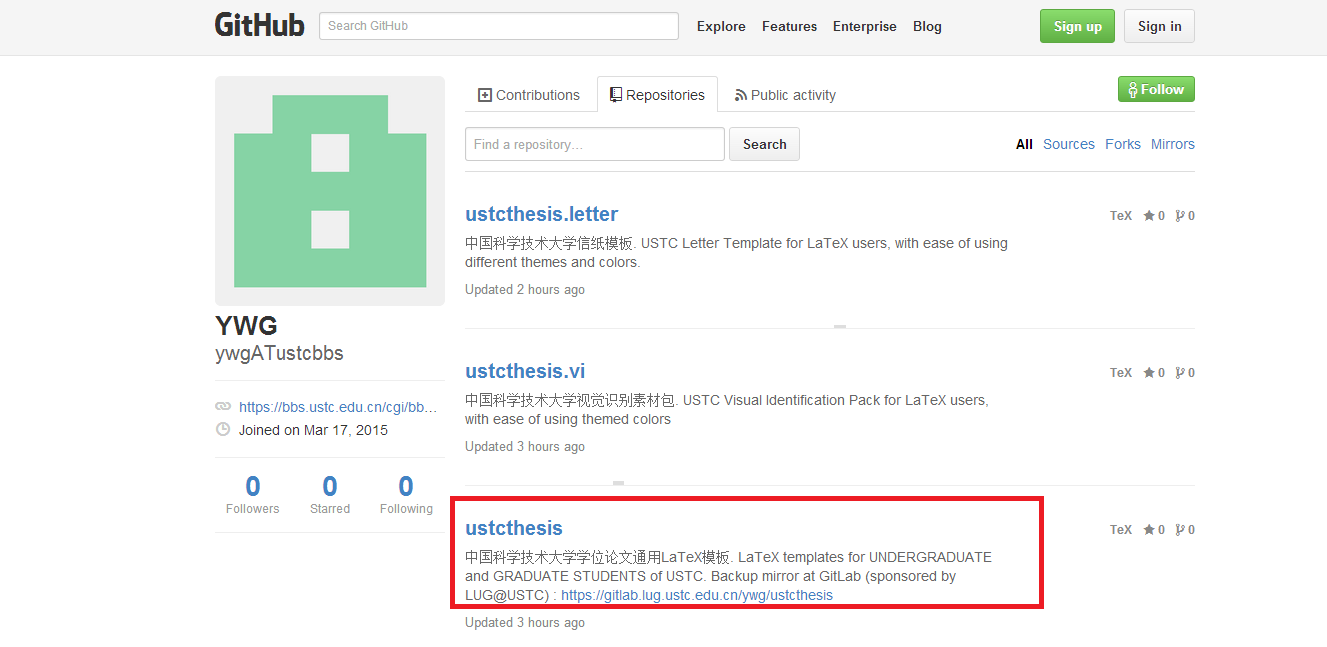
\includegraphics[width=0.48\textwidth]{download}
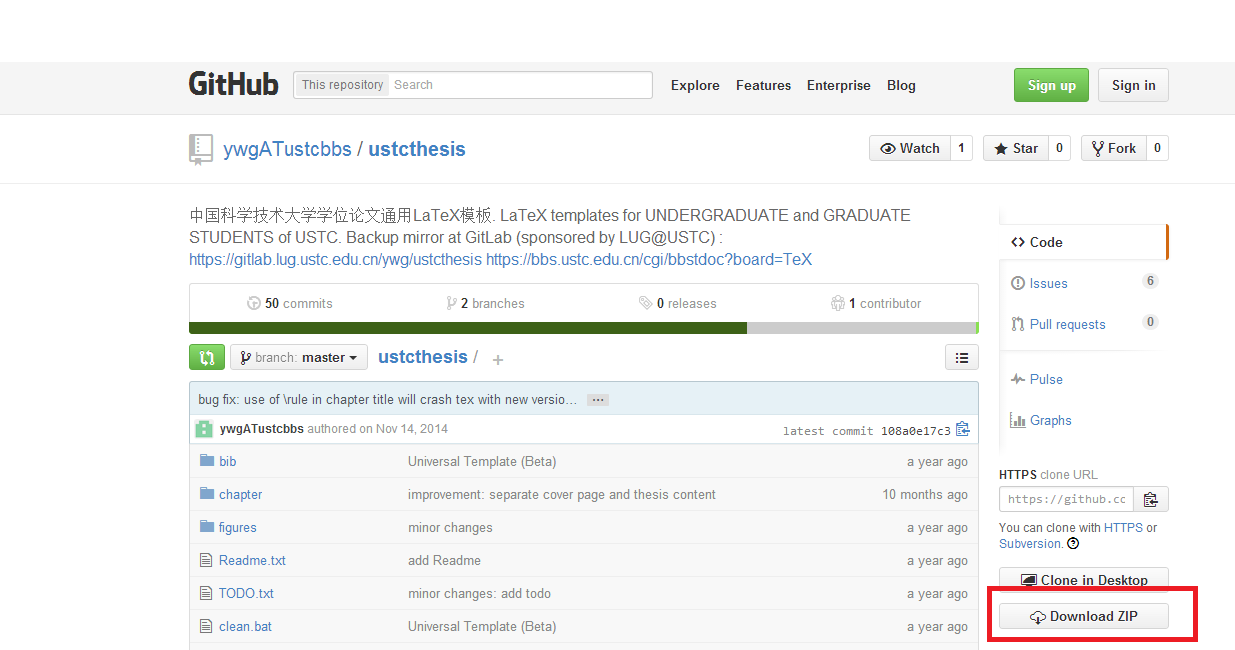
\includegraphics[width=0.48\textwidth]{download1}
\figcaption{在GitHub上进行模板下载}
\label{fig:download}
\end{figure}

\textbf{特别注意1:}本硕博通用论文模板的名称为ustcthesis,其他项目如ustcthesis.vi/ustcthesis.letter/ustcthesis.beamer是用作其他用途的模板,并非本模板所需文件,如对其感兴趣,请进入对应页面了解详情。

\textbf{特别注意2:}此前开发的本科和硕博模板已暂停支持,但仍然可以选择对应的版本(ustcthesis.bachelor和ustcthesis.msphd)进行下载。

模板的安装使用方法有多种,最为简单便捷的方法是直接解压缩下载好的压缩包,修改其中的main.tex文件以及chapter文件夹下的文件,必要时增加所需要的文件。需要注意的是确保所有文件使用UTF-8编码。Windows系统中将其他编码的文件转化为UTF-8的方法是: 用记事本打开这些文件, 然后点击文件—另存为—在最下方选择UTF-8 编码。

\subsection{\texorpdfstring{\LaTeX}{LaTeX}系统的安装和使用}
由于本模板使用了较多的宏包,因此建议使用TeXLive2013及以上版本的\LaTeX 发行版。TeXLive2013可以在Windows、GNU/Linux和大多数Unix系统中运行。对于MacOSX,推荐使用MacTeX-2013。详细信息参考\url{https://www.tug.org/texlive/}。

对于中国科学技术大学的校内用户而言,最方便的获取TeXLive2013的途径是使用LUG@USTC提供的CTAN镜像源(\url{http://mirrors.ustc.edu.cn/CTAN/})。最新的TeXLive位于/CTAN/systems/texlive/目录(\url{http://mirrors.ustc.edu.cn/CTAN/systems/texlive/})内。用户可以选择进入Images文件夹下载完整的光盘并刻录安装,也可以选择进入tlnet文件夹下载运行install-tl.exe进行在线安装。需要注意的是,在线安装的时候可以通过切换安装源为本校镜像源来加快下载安装速度。

对于校外用户,可以通过CTAN.org获得官方的TeXLive。CTAN在全球41个国家和地区分布有115个镜像站点,它们的地址可以在\url{http://www.ctan.org/mirrors/}找到。

\subsection{推荐使用的编辑器}
\LaTeX 的源文件是一个或多个文本文件,这意味着可以使用最为简单的文本编辑器来撰写论文。但是和许多编程语言类似,使用一款带有语法高亮、命令补全等功能的文本编辑器能够大大提升协作效率。

对于不同的编辑器而言,能够实现的功能也不尽相同,加之不同用户拥有不同的使用习惯,简单武断的说某一款编辑器好或者不好有失公允。对于\TeX 写作而言,用户使用的编辑器大致可以分为两类:通用的文本编辑器和专用的GUI编辑器。通用的文本编辑器中公认比较好用的有Vim(Linux)、Emacs(Linux)、Notepad++(Windows)等等\footnote{当然,这些软件可能都有跨平台版本,而且也有其他很多优秀的文本编辑器,不要在意这些细节啦,我并不想挑起编辑器的圣战。:P}。这些编辑器有着强大的功能,但是往往需要在编辑和编译之间来回切换。而专用的GUI编辑器如TeXShop(Mac)、TeXWorks(windows/Linux)和Winedit(Windows、付费软件)等虽然可能在文本编辑上略显笨拙,但是其优点在于编写和生成一体化,简单化。

使用何种编辑器这个问题见仁见智,但是对于一个刚从word转来的新人,从界面简洁、操作简单、功能实用的角度出发,TeXWorks不失为一款优秀的GUI软件,如\autoref{fig:texworks}。

\begin{figure}
\centering
\includegraphics[width=0.9\textwidth]{texworks}
\figcaption{TeXWorks主界面}
\label{fig:texworks}
\end{figure}

Windows系统下TeXWorks的界面拥有左右两个窗口,左边为编辑窗口,右边为预览窗口,当编辑完文档之后,只需点击绿色的开始按钮,就可以立即对文档进行保存并编译,可以选择不同的引擎进行处理。编译过程中的信息会在左侧窗口下方显示。TeXWorks默认UTF-8编码,安装时自动查找TeX安装目录,支持自动缩进、语法高亮、命令补全、正则式查找以及TeX文件和PDF的正反查找(即点击命令跳转到对应pdf文字位置以及点击pdf文字跳转到对应命令,操作是Ctrl+单击)。这些功能对新手来说都是十分友好的。

\section{问题反馈}

如果您在使用过程中有疑问,遇到困难,可以在\href{http://bbs.ustc.edu.cn/cgi/bbsdoc?board=TeX}{瀚海星云\TeX{}讨论区}或者相关的\LaTeX 论坛(如\href{http://bbs.ctex.org}{CTEX 论坛})寻求帮助,但是请注意遵守论坛的各项规定。

如果使用过程中遇到Bug,请提交到\href{http://bbs.ustc.edu.cn/cgi/bbsdoc?board=TeX}{瀚海星云\TeX{}讨论区},或者提交到相应的\href{http://code.google.com/p/ustcthesis/issues/list}{Google UstcThesis Project(http://code.google.com/p/ustcthesis/issues/list)},请注明是什么版本模板的bug。
  % \chapter{模板的基础使用说明}

\section{模板基本说明}
使用本模板,您应首先具备基本的\LaTeX 知识,如果您刚刚接触\LaTeX,建议您先学习相关的用户文档或教程。

模板文件名为ustcthesis.cls。方便起见,将该文件放置在与论文主文件同一文件夹中即可。如果需要使用增强功能,模板提供了一个名为ustcxtra.cls的补充包。将该文件放置在与论文主文件同一文件夹中即可。

模板提供一个文档类ustcthesis,使用\verb|\documentclass{ustcthesis}|来加载模板。

模板可以使用ctexbook文档类的相应选项,默认加载的是 cs4size, a4paper, fancyhdr, fntef。需要注意的是默认加载 \emph{双面/章节从奇数页开始} 选项,如果需要\emph{单面} 选项,请使用:
\begin{Code}
\documentclass[<学位>,oneside,openany]{ustcthesis}
\end{Code}

\begin{table}[htp]
\centering
\tabcaption{模板提供的新文档选项}
\label{tab:newdocopt}
\begin{tabular}{lL{5cm}L{4cm}}
\toprule
文档选项&说明&备注\tabularnewline
\midrule
bachelor	&学士				&\multirow{3}{4cm}{指明论文类型,不能同时存在}\tabularnewline
master		&硕士				&\tabularnewline
doctor		&博士				&\tabularnewline
basic		&仅使用基础功能	&此时无法使用增强包中的命令\tabularnewline
oldfontcfg	&使用老版本的硕博论文模板的字体设置			&需要补充包\tabularnewline
euler		&使用euler数学字体&需要补充包\tabularnewline
adobefont	&使用adobe的字体	&\multirow{2}{4cm}{仅仅防止误输入}\tabularnewline
adobefonts	&使用adobe的字体	&\tabularnewline
notchinese	&使用外文撰写论文	Use this option to write thesis in other laguage(s)& If you use language(s) other than Chinese and English, you should refer to \autoref{tab:newcmd}. \tabularnewline
\bottomrule
\end{tabular}
\end{table}

\subsection{模板推荐加载设置}
推荐使用如下选项加载模板:
\begin{Code}
\documentclass[<学位>,euler,twoside,openright]{ustcthesis}
\end{Code}

如果缺少大多数宏包,建议使用
\begin{Code}
\documentclass[<学位>,basic,twoside,openright]{ustcthesis}
\end{Code}

\section{模板提供的新环境和命令}
模板提供了若干个新环境和命令,如\autoref{tab:newenv}和\autoref{tab:newcmd}所列,这些新环境和命令有的比较简单,有的则附有对应的示例。

\begin{longtable}{lll}%@{\extracolsep{\fill}}
\caption[模板提供的新环境]{模板提供的新环境}
\label{tab:newenv} \\
\toprule
名称  & 说明 & 备注\tabularnewline\midrule
\endfirsthead
\bottomrule
\endfoot
\caption[模板提供的新环境(续)]{模板提供的新环境(续)} 
\label{tab:newenv2} \\
\toprule
名称  & 说明 & 备注\tabularnewline\midrule
\endhead
\bottomrule
\endlastfoot
enabstract&英文摘要&\tabularnewline
cnabstract&中文摘要&\tabularnewline
thanks&致谢&\tabularnewline
denotation&主要符号对照表&需要ustcxtra,用法见./chapter/denotation.tex\tabularnewline
Code&代码&需要ustcxtra,效果见\autoref{codex}\tabularnewline
Codex&代码&需要ustcxtra,效果见\autoref{codex}\tabularnewline
CodeScript&代码&需要ustcxtra,效果见\autoref{codex}\tabularnewline
CodexScript&代码&需要ustcxtra,效果见\autoref{codex}\tabularnewline
code&代码&需要ustcxtra,效果未测试\tabularnewline
theorem &定理&\tabularnewline
lemma &引理&\tabularnewline
example &例&\tabularnewline
algorithm &算法&\tabularnewline
definition &定义& \tabularnewline
axiom &公理 &\tabularnewline
property &性质 & \tabularnewline
proposition &命题 &\tabularnewline
corollary& 推论 &\tabularnewline
remark &注解  &\tabularnewline
condition &条件 & \tabularnewline
conclusion &结论 & \tabularnewline
assumption &假设 & \tabularnewline
prove &证明 &\tabularnewline
proof&证明 &与prove的区别见\autoref{pic:proofandprove}\tabularnewline
\end{longtable}

\begin{longtable}{lp{0.35\textwidth}p{0.35\textwidth}}%@{\extracolsep{\fill}}
\caption[模板提供的新命令]{模板提供的新命令}
\label{tab:newcmd} \\
\toprule
名称  & 说明 & 备注\tabularnewline\midrule
\endfirsthead
\bottomrule
\endfoot
\caption[模板提供的主要新命令(续)]{模板提供的主要新命令(续)} 
\label{tab:newcmd2} \\
\toprule
名称  & 说明 & 备注\tabularnewline\midrule
\endhead
\bottomrule
\endlastfoot
\textbackslash chuhao\{\}&字号:初号&类似的有:\textbackslash yihao\{\}...\textbackslash qihao\{\}\tabularnewline
\textbackslash xiaochu\{\}&字号:小初号&类似的有:\textbackslash xiaoer\{\}...\textbackslash xiaowu\{\}\tabularnewline
\textbackslash xiaochuhao\{\}&字号:小初号&类似的有:\textbackslash xiaoerhao\{\}...\textbackslash xiaowuhao\{\}\tabularnewline
\textbackslash ustclofname\{\}&定义图表索引名称&需在\textbackslash ustclof前使用\tabularnewline
\textbackslash ustclof&生成图表索引并加入目录&\tabularnewline
\textbackslash ustclotname\{\}&表格索引名称&与\textbackslash ustclofname\{\}类似\tabularnewline
\textbackslash ustclot&表格索引&与\textbackslash ustclot类似\tabularnewline
\textbackslash ustcloaname\{\}&算法索引名称&需要ustcxtra,与\textbackslash ustclofname\{\}类似\tabularnewline
\textbackslash ustcloa&算法索引&需要ustcxtra,与\textbackslash ustclof类似\tabularnewline
\textbackslash title\{\}&标题&中文\tabularnewline
\textbackslash author\{\}&作者&中文\tabularnewline
\textbackslash advisor\{\}&导师&中文\tabularnewline
\textbackslash coadvisor\{\}&第二导师&中文,可留空\tabularnewline
\textbackslash major\{\}&专业&硕博全称,本科不需要\tabularnewline
\textbackslash depart\{\}&院系&硕博代号,本科全称\tabularnewline
\textbackslash submitdate\{\}&完成日期&中文\tabularnewline
\textbackslash en...\{\}&由title至submitdate&以上命令的英文版本\tabularnewline
\textbackslash studentid\{\}&学号&仅本科需要\tabularnewline
\textbackslash spinetitle\{\}&书脊使用的标题&在\textbackslash title中含有部分控制命令时使用\tabularnewline
\textbackslash keywords\{\}&中文关键词&在cnabstract中使用\tabularnewline
\textbackslash enkeywords\{\}&英文关键词&在enabstract中使用\tabularnewline
\textbackslash figcaption\{\}&图形标题&无论是否在图形环境中均可得到正确标题\tabularnewline
\textbackslash tabcaption\{\}&&与上类似,表格用\tabularnewline
C\{width\}&定宽居中&表格环境中p\{width\}的加强,参考\autoref{tab:tblcmp}\tabularnewline
L\{width\}&定宽左齐&\tabularnewline
R\{width\}&定宽右齐&\tabularnewline
\textbackslash scite\{\}&上标引用&\tabularnewline
\textbackslash song&宋体&另有其他,详见ustcxtra\tabularnewline
\textbackslash upGamma&立直希腊Gamma&另有其他,详见ustcxtra\tabularnewline

\textbackslash otherustcstr  & 'University of Science and Technology of China'. A translation of this string in your own language. \emph{Only useful when you are writting a thesis in language(s) other than Chinese and English}. &  According to regulations of USTC, your need to put three title pages: Chinese, English and your own language title pages. So use these commands to generate the third title page. \tabularnewline%
\textbackslash otherthesisstr  & 'A dissertation for bachelor(/master/doctor)'s degree' & Similar to previous one \tabularnewline%
\textbackslash otherauthorstr  & 'Author' & Similar to previous one \tabularnewline%
\textbackslash otherdepartmentstr  & 'Department' & Similar to previous one \tabularnewline%
\textbackslash otherstudentidstr  & 'Student ID' & Similar to previous one \tabularnewline%
\textbackslash othersupervisorstr  & 'Supervisor' & Similar to previous one \tabularnewline%
\textbackslash otherfinishedtimestr  & 'Finished Time' & Similar to previous one \tabularnewline%
\textbackslash otherspecialitystr  & 'Speciality' & Similar to previous one \tabularnewline%
\textbackslash othertitle  & Thesis title. Put your thesis title in your own language here. \emph{Only useful when you are writting a thesis in language(s) other than Chinese and English}. &   \tabularnewline
\textbackslash otherauthor  & Your name & Similar to previous one \tabularnewline
\textbackslash otheradvisor  & Your advisor's name & Similar to previous one \tabularnewline
\textbackslash othercoadvisor  & Co-advisor & Similar to previous one \tabularnewline
\textbackslash othersubmitdate  & Thesis submit date & Similar to previous one \tabularnewline
\textbackslash othermajor  & Your major & Similar to previous one \tabularnewline
\textbackslash otherdepart  & Your department & Similar to previous one \tabularnewline
\end{longtable}

需要注意的是,这里prove环境翻译为“证明”,事实上,其实prove环境不是用作theorem等类似环境配套证明的,prove环境是与theorem等环境同级别的环境。与theorem等环境相配套的证明环境是proof环境。使用时请注意下两个环境的差异:proof环境是没有编号的,是与theorem这类环境配合使用的;prove环境是有编号的,更多的是类似于证明题的题目。详细的差别见\autoref{pic:proofandprove}。

\begin{figure}
\centering
  \framebox{\includegraphics[scale=1]{figures/proofandprove}}
  \figcaption{proof、prove以及部分其他数学环境的差异}
  \label{pic:proofandprove}
\end{figure}

\section{使用模板的一些建议}

公式、章节、图和表格等(不包括脚注和参考文献)的交叉引用可以使用\verb|\autoref{label}|来得到正确的引用。例如使用\verb|\autoref{some_pic}|可以得到“图 X”的引用,使用\verb|\autoref{some_table}|可以得到“表 X”的引用。

建议使用\verb|\figcaption{}|命令得到所有图形的标题,表格也是。这样无论是否在图形环境中均能够得到正确的带图/表编号的标题,而在图形环境之外使用\verb|\caption{}|命令会报错。

%封面是按照制本厂的要求制作的,其中行宽和行高都是固定的,中文标题最多占两行,英文标题最多占三行。如果您的题目超过了这个限制,请缩减题目长度,不要擅自修改模板中的相关配置参数。


  % 
\chapter{代码示例}
\label{chap:example}
\section{Euler数学字体示例}
$$
abcdefghijklmnopqrstuvwxyz
$$
$$
ABCDEFGHIJKLMNOPQRSTUVWXYZ
$$
$$
0123456789
$$
\begin{equation}
\begin{split}
\{S_i=0\}=\frac{a_i}{b_i+a_i} \\
\{S_i=1\}=\frac{b_i}{b_i+a_i} \label{1}
\end{split}
\end{equation}

\section{上标引用示例}
\verb|\scite{lshort-cn}|,效果\scite{lshort-cn}。

\section{表格环境加强命令示例}
本模板提供了表格环境下p\{width\}加强版命令,使用L\{width\}等可以在指定宽度的同时指定对齐方式。

\begin{minipage}{\textwidth}
\begin{Codex}[numbers=left]
\begin{table}
\tabcaption{几种命令效果对比的对比}
\label{tab:tblcmp}
\centering
\begin{tabular}{c||l|c|r|p{2.5cm}|L{2.5cm}|C{2.5cm}|R{2.5cm}}
\hline
命令&l&c&r&p\{width\}&L\{width\}&C\{width\}&R\{width\}\\
\hline
效果&左齐&居中&右齐&定宽&左齐定宽&居中定宽&右齐定宽\\
\hline
\end{tabular}
\end{table}
\end{Codex}

\tabcaption{几种命令效果对比的对比}
\label{tab:tblcmp}
\centering
\begin{tabular}{c||l|c|r|p{2.5cm}|L{2.5cm}|C{2.5cm}|R{2.5cm}}
\hline
命令&l&c&r&p\{width\}&L\{width\}&C\{width\}&R\{width\}\\
\hline
效果&左齐&居中&右齐&定宽&左齐定宽&居中定宽&右齐定宽\\
\hline
\end{tabular}
\end{minipage}

\section{自定义代码环境示例}
\label{codex}
\subsection{Code环境}
\begin{minipage}{\textwidth}
\begin{minipage}{0.4\textwidth}
\begin{Code}[label=a.cpp, numbers=left]
This is Code environment
A simple example.
For more options, see fancyvrb's manual.
\end{Code}
\end{minipage}
\hfill\begin{minipage}{0.4\textwidth}
\begin{Verbatim}[fontsize=\scriptsize,baselinestretch=0.9,xleftmargin=3mm,frame=lines,labelposition=all,framesep=5pt]
\begin{Code}[label=a.cpp, numbers=left]
This is Code environment
A simple example.
For more options, see fancyvrb's manual.
\end{Code}
\end{Verbatim}
\end{minipage}
\end{minipage}

\subsection{Codex环境}
\begin{minipage}{\textwidth}
\begin{minipage}{0.4\textwidth}
\begin{Codex}[label=a.cpp, numbers=left]
This is Codex environment
A simple example.
For more options, see fancyvrb's manual.
\end{Codex}
\end{minipage}
\hfill\begin{minipage}{0.4\textwidth}
\begin{Verbatim}[fontsize=\scriptsize,baselinestretch=0.9,xleftmargin=3mm,frame=lines,labelposition=all,framesep=5pt]
\begin{Codex}[label=a.cpp, numbers=left]
This is Codex environment
A simple example.
For more options, see fancyvrb's manual.
\end{Codex}
\end{Verbatim}
\end{minipage}
\end{minipage}

\subsection{CodeScript环境}
\begin{minipage}{\textwidth}
\begin{minipage}{0.4\textwidth}
\begin{CodeScript}[label=a.cpp, numbers=left]
This is CodeScript environment
A simple example.
For more options, see fancyvrb's manual.
\end{CodeScript}
\end{minipage}
\hfill\begin{minipage}{0.4\textwidth}
\begin{Verbatim}[fontsize=\scriptsize,baselinestretch=0.9,xleftmargin=3mm,frame=lines,labelposition=all,framesep=5pt]
\begin{CodeScript}[label=a.cpp, numbers=left]
This is CodeScript environment
A simple example.
For more options, see fancyvrb's manual.
\end{CodeScript}
\end{Verbatim}
\end{minipage}
\end{minipage}

\subsection{CodexScript环境}
\begin{minipage}{\textwidth}
\begin{minipage}{0.4\textwidth}
\begin{CodexScript}[label=a.cpp, numbers=left]
This is CodexScript environment
A simple example.
For more options, see fancyvrb's manual.
\end{CodexScript}
\end{minipage}
\hfill\begin{minipage}{0.4\textwidth}
\begin{Verbatim}[fontsize=\scriptsize,baselinestretch=0.9,xleftmargin=3mm,frame=lines,labelposition=all,framesep=5pt]
\begin{CodexScript}[label=a.cpp, numbers=left]
This is CodexScript environment
A simple example.
For more options, see fancyvrb's manual.
\end{CodexScript}
\end{Verbatim}
\end{minipage}
\end{minipage}

\section{表格示例}
具体代码请参考源文件./chapter/chap-example.tex。
\begin{table}[htbp]
\centering
\caption{基于因子分析的失配补偿结果}
\label{tab:jfa-gmm-ubm}
\begin{tabular}{cccccc}
    \toprule
    &\multirow{2}{*}{\#Mix}&\multicolumn{2}{c}{No-norm}
    &\multicolumn{2}{c}{Tnorm}\\
    \cline{3-4} \cline{5-6}
		&		& EER(\%) 	& MinDCF & EER(\%) 	& MinDCF\\
    \midrule
	\multirow{3}{*}{GMM-UBM}
    &256 		& 12.43 	& 0.0647	& 12.85    & 0.0580\\
    &512 		& 10.02 	& 0.0464	& 8.88 	   & 0.0370\\
    &1024 		& 9.97 	    & 0.0457	& 8.72 	   & 0.0372\\
    \midrule
	\multirow{3}{*}{Factor Analysis}
    &256 		& 8.09 	& 0.0331 	& 7.39 	& 0.0319\\
    &512 		& 7.08 	& 0.0305 	& 6.53 	& 0.0292\\
    &1024 		& 6.83 	& 0.0295 	& \textbf{6.29} 	& \textbf{0.0279}\\
 \bottomrule
\end{tabular}
\end{table}

\section{算法示例}
具体代码请参考源文件./chapter/chap-example.tex。
\IncMargin{1em}
\begin{algorithm}
\SetKwData{Left}{left}\SetKwData{This}{this}\SetKwData{Up}{up}
\SetKwFunction{Union}{Union}\SetKwFunction{FindCompress}{FindCompress}
\SetKwInOut{Input}{input}\SetKwInOut{Output}{output}
\Input{$O_t,UBM,U$}
\Output{$x,y$}
\BlankLine
\emph{$y\leftarrow 0;$$x_h\leftarrow 0;$$h=1,...,H$ }\;
\For{$i=1$ \KwTo Number of E-M iterations}{
\emph{E Step}:\\
\For{$h=1$ \KwTo $H$}{\label{forins}
对于每一条语音段,计算其EM统计量(零阶统计量$N_h$,一阶统计量$S_{X,h}$\;
}
计算每一个人所有语音段的零阶统计量$N$\\
计算每一个人所有语音段的一阶统计量$S$\\
\emph{M Step}:\\
\For{$j=1$ \KwTo Number of Gauss-Seidel iterations}{
\For{$h=1$ \KwTo $H$}{\label{forins}
估计每一语音段$h$的失配因子$x_h$
}
估计模型的话者因子$y$
}
}
\Return{$\mu = m+Dy$}
\caption{disjoint decomposition}\label{algo_disjdecomp}
\end{algorithm}\DecMargin{1em}

\section{引用参考文献示例}
参考文献测试:\citep{deng:01a}
  \chapter{第一章 绪论}
\label{chap:introduction}

本章

\section{系统要求}
\subsection{系统要求}
本模板基于\CTeX 的ctexbook文档类进行定制,基于\XeTeX 引擎排版。使用本模板的最基础功能时,除了上述需求外,还需要如下几类宏包(直接引用):
\begin{description}
\item[数学类]{amsmath、amsthm、amsfonts、amssymb、bm}
\item[格式类]{titletoc、titlesec、geometry、caption}
\item[表格类]{multicol、multirow}
\item[其他]{xparse、xeCJK、hyperref、natbib、subfiles}
\end{description}
可能有部分宏包是由上述宏包以及\CTeX 间接引用的,此处不一一列举。

另外,如果需要使用增强的ustcxtra.cls,额外需要如下宏包(直接引用):
\begin{description}
\item[默认载入]{times、algorithm2e、graphicx、psfrag、subfig、enumerate、epsfig、float、paralist、booktabs、footmisc、wasysym、longtable、bbm、indentfirst、ifthen、caption3、array、fancyvrb、xcolor、url}
\item[条件载入]{eulervm(仅在文档类处于增强模式并在文档类选项注明euler时载入)}
\end{description}

\section{下载与安装}
\subsection{模板文件清单}
使用模板之前请确保模板文件没有缺失损坏。文件清单如\autoref{tab:filelist},标注关键的文件需要确保文件以及路径的完整。
\begin{table}[htp]
\centering
\tabcaption{模板主要文件清单}
\label{tab:filelist}
\begin{tabular}{lll}
\toprule
文件名&相对路径&备注\tabularnewline
\midrule
clean.bat			&./			&清理脚本\tabularnewline
clean.sh			&./			&清理脚本\tabularnewline
main.pdf			&./			&示例文件\tabularnewline
main.tex 			&./			&示例TeX文件\tabularnewline
make.bat			&./			&生成脚本\tabularnewline
make.sh				&./			&生成脚本\tabularnewline
ustcbib.bst		&./			&Bib格式文件\tabularnewline
ustcthesis.cls		&./			&(关键)模板\tabularnewline
ustcxtra.cls		&./			&(关键)模板增强\tabularnewline
ustc\_logo\_fig.eps	&./figures	&(关键)科大校徽\tabularnewline
ustc\_logo\_text.eps&./figures	&(关键)科大校名\tabularnewline
\bottomrule
\end{tabular}
\end{table}

\subsection{模板下载与使用}
由于Google公司决定停止Google Code服务,故原Google Code项目网站的模板整体迁移至GitHub网站并继续进行更新维护。本模板及本示例文件可以在GitHub网
站\url{https://github.com/ywgATustcbbs?tab=repositories}下载。备份托管地址为\url{https://gitlab.lug.ustc.edu.cn/ywg/ustcthesis},此托管网站由LUG@USTC提供服务。

请在项目页面选择ustcthesis->新页面中选择Download Zip下载最新模板文件(\autoref{fig:download})。也可以通过git clone的方式获得模板。

\begin{figure}
\centering
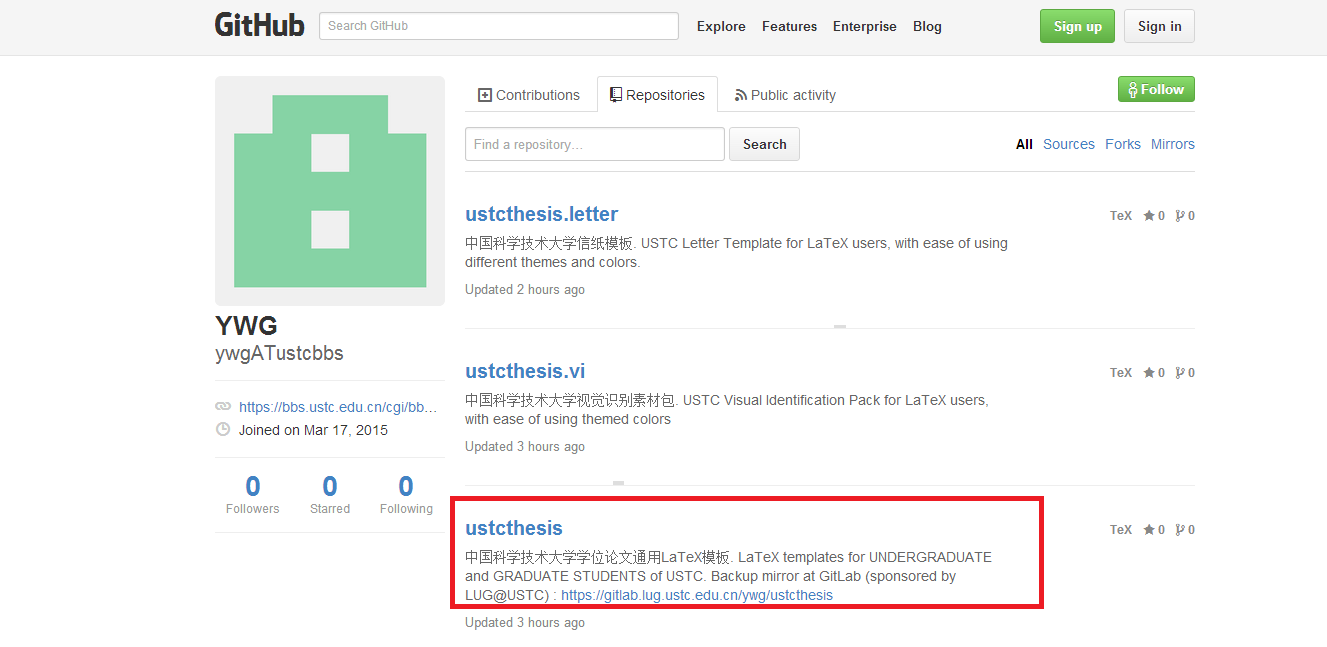
\includegraphics[width=0.48\textwidth]{download}
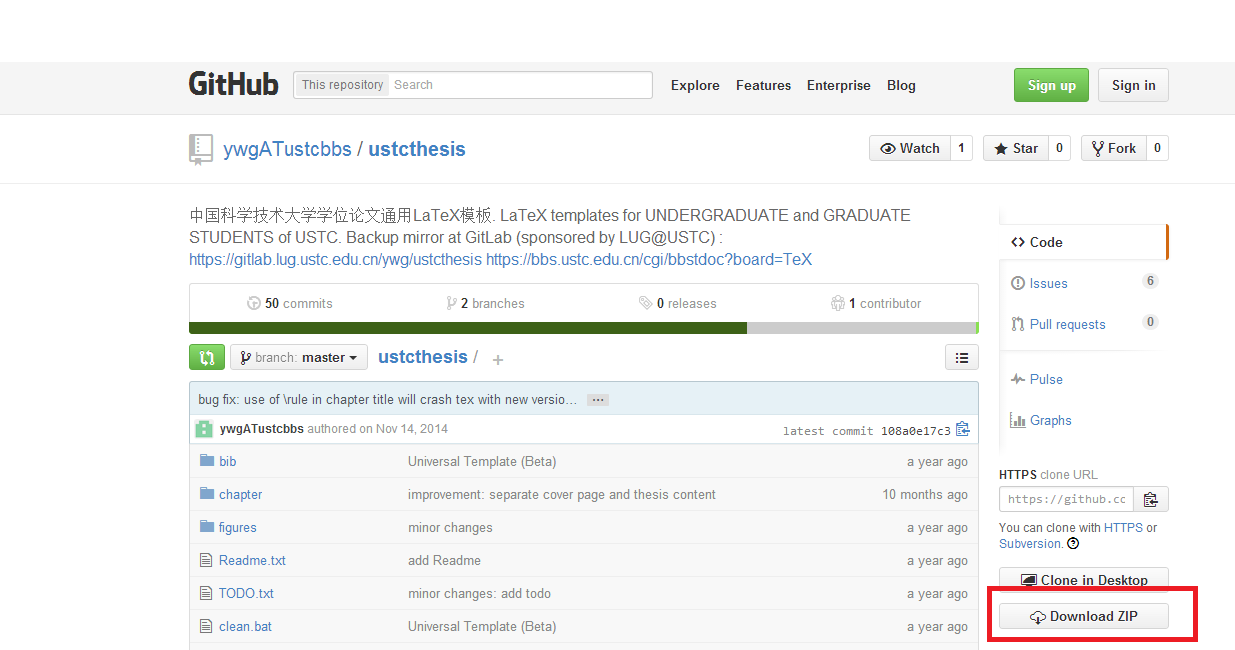
\includegraphics[width=0.48\textwidth]{download1}
\figcaption{在GitHub上进行模板下载}
\label{fig:download}
\end{figure}

\textbf{特别注意1:}本硕博通用论文模板的名称为ustcthesis,其他项目如ustcthesis.vi/ustcthesis.letter/ustcthesis.beamer是用作其他用途的模板,并非本模板所需文件,如对其感兴趣,请进入对应页面了解详情。

\textbf{特别注意2:}此前开发的本科和硕博模板已暂停支持,但仍然可以选择对应的版本(ustcthesis.bachelor和ustcthesis.msphd)进行下载。

模板的安装使用方法有多种,最为简单便捷的方法是直接解压缩下载好的压缩包,修改其中的main.tex文件以及chapter文件夹下的文件,必要时增加所需要的文件。需要注意的是确保所有文件使用UTF-8编码。Windows系统中将其他编码的文件转化为UTF-8的方法是: 用记事本打开这些文件, 然后点击文件—另存为—在最下方选择UTF-8 编码。

\subsection{\texorpdfstring{\LaTeX}{LaTeX}系统的安装和使用}
由于本模板使用了较多的宏包,因此建议使用TeXLive2013及以上版本的\LaTeX 发行版。TeXLive2013可以在Windows、GNU/Linux和大多数Unix系统中运行。对于MacOSX,推荐使用MacTeX-2013。详细信息参考\url{https://www.tug.org/texlive/}。

对于中国科学技术大学的校内用户而言,最方便的获取TeXLive2013的途径是使用LUG@USTC提供的CTAN镜像源(\url{http://mirrors.ustc.edu.cn/CTAN/})。最新的TeXLive位于/CTAN/systems/texlive/目录(\url{http://mirrors.ustc.edu.cn/CTAN/systems/texlive/})内。用户可以选择进入Images文件夹下载完整的光盘并刻录安装,也可以选择进入tlnet文件夹下载运行install-tl.exe进行在线安装。需要注意的是,在线安装的时候可以通过切换安装源为本校镜像源来加快下载安装速度。

对于校外用户,可以通过CTAN.org获得官方的TeXLive。CTAN在全球41个国家和地区分布有115个镜像站点,它们的地址可以在\url{http://www.ctan.org/mirrors/}找到。

\subsection{推荐使用的编辑器}
\LaTeX 的源文件是一个或多个文本文件,这意味着可以使用最为简单的文本编辑器来撰写论文。但是和许多编程语言类似,使用一款带有语法高亮、命令补全等功能的文本编辑器能够大大提升协作效率。

对于不同的编辑器而言,能够实现的功能也不尽相同,加之不同用户拥有不同的使用习惯,简单武断的说某一款编辑器好或者不好有失公允。对于\TeX 写作而言,用户使用的编辑器大致可以分为两类:通用的文本编辑器和专用的GUI编辑器。通用的文本编辑器中公认比较好用的有Vim(Linux)、Emacs(Linux)、Notepad++(Windows)等等\footnote{当然,这些软件可能都有跨平台版本,而且也有其他很多优秀的文本编辑器,不要在意这些细节啦,我并不想挑起编辑器的圣战。:P}。这些编辑器有着强大的功能,但是往往需要在编辑和编译之间来回切换。而专用的GUI编辑器如TeXShop(Mac)、TeXWorks(windows/Linux)和Winedit(Windows、付费软件)等虽然可能在文本编辑上略显笨拙,但是其优点在于编写和生成一体化,简单化。

使用何种编辑器这个问题见仁见智,但是对于一个刚从word转来的新人,从界面简洁、操作简单、功能实用的角度出发,TeXWorks不失为一款优秀的GUI软件,如\autoref{fig:texworks}。

\begin{figure}
\centering
\includegraphics[width=0.9\textwidth]{texworks}
\figcaption{TeXWorks主界面}
\label{fig:texworks}
\end{figure}

Windows系统下TeXWorks的界面拥有左右两个窗口,左边为编辑窗口,右边为预览窗口,当编辑完文档之后,只需点击绿色的开始按钮,就可以立即对文档进行保存并编译,可以选择不同的引擎进行处理。编译过程中的信息会在左侧窗口下方显示。TeXWorks默认UTF-8编码,安装时自动查找TeX安装目录,支持自动缩进、语法高亮、命令补全、正则式查找以及TeX文件和PDF的正反查找(即点击命令跳转到对应pdf文字位置以及点击pdf文字跳转到对应命令,操作是Ctrl+单击)。这些功能对新手来说都是十分友好的。

\section{问题反馈}

如果您在使用过程中有疑问,遇到困难,可以在\href{http://bbs.ustc.edu.cn/cgi/bbsdoc?board=TeX}{瀚海星云\TeX{}讨论区}或者相关的\LaTeX 论坛(如\href{http://bbs.ctex.org}{CTEX 论坛})寻求帮助,但是请注意遵守论坛的各项规定。

如果使用过程中遇到Bug,请提交到\href{http://bbs.ustc.edu.cn/cgi/bbsdoc?board=TeX}{瀚海星云\TeX{}讨论区},或者提交到相应的\href{http://code.google.com/p/ustcthesis/issues/list}{Google UstcThesis Project(http://code.google.com/p/ustcthesis/issues/list)},请注明是什么版本模板的bug。
  \chapter{相关技术背景及算法}
\label{chap:algorithm}

\begin{figure}[ht]
\centering
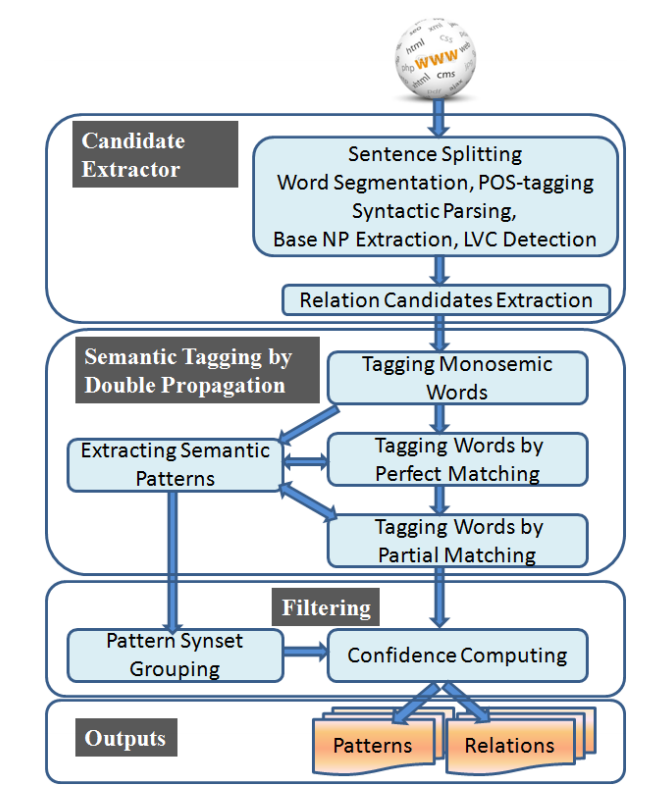
\includegraphics[width=10cm]{ZORE}
\caption{ZORE 体系结构}\label{fig:ZORE}
\end{figure}

\section{ZORE 的简介}
ZORE 的体系结构如图 ~\ref{fig:ZORE} 所示。它由三个部件组成。第一个部件是候选关系提取器,这个提取器获取输入的文本然后进行句子的分割、字词的分割、添加 POS 标签、句法解析、基本的 NP(noun phrase,名词短语) 提取、轻量化的动词结构(LVC,light verb structure)探测和候选关系提取。它的输出是所有候选关系的集合。第二个部件对关系进行添加标签,然后通过双重拓展算法提取语义模式。第三个部件则将被提取出的模式进行同义词集分组,关系则依据“可信分数”进行过滤。

\subsection{提取候选关系}

\subsubsection{解析与基本的 NP 提取}
ZORE 通过应用一系列的 NLP(Natural Language Process,自然语言处理)工具对输入的文本进行流水线处理来分析句法结构。每个句子都通过 Stanford 分割器\citep{chang2008}被分割为一个字词列表,并通过 ZPar \citep{zhang2011}来进行解析,通过标准 CTB \citep{xue2005}来添加 POS 标志和分析结构组成。并对最后生成的构成树使用 Stanford 解析器\citep{chang2008}将其变形为有 Stanford dependencies 的投影树。

接下去,基本的 NPs (名词短语)从依赖树中被提取出来,在这里基本 NP 是一个最大短语,其字词只能拥有来自表 ~\ref{tab:NP} 第一行的 POS。基本 NP 的核心词语可以是一个名词,一个代词,一个数字或是一个量词(表 ~\ref{tab:NP} 的第二行)。基本 NP 里的依赖标签只能来自表 ~\ref{tab:NP} 的第三行。所以,很明显的,一个基本 NP 并不包含其他的基本 NP,并且它本身也不被其他的基本 NP 所包含。

\begin{longtable}{cc}
% 首页表头
\caption[基本 NP 标志表]{包含了 POS 标志和依赖标签,在前三行的标签被用来进行基本 NP 的提取,而最后一行中的标签用于从基本 NP 遍历到谓词短语} \label{tab:NP} \\
\toprule[1.5pt]
  & 标志\\
\midrule[1pt]
\endfirsthead
% 续页表头
\caption[]{(续)} \\
\toprule[1.5pt]
  & 标志\\
\midrule[1pt]
\endhead
% 首页表尾
\hline
\multicolumn{2}{r}{\small 续下页}
\endfoot
% 续页表尾
\bottomrule[1.5pt]
\endlastfoot
基本 NP 修饰语   &   NN (common noun), M (measure word), \\
    &   CD (cardinal number), OD (ordinal number),\\
    &   PN (pronoun), NR(proper noun),\\
    &   NT (temporal noun), \\
    &   JJ (other noun-modifier), or PU (punctuation) \\
    \hline
基本 NP 中的标签  &   nn (noun compound modifier), conj (conjunct),\\
    &   nummod (number modifier),\\
    &   cc (coordinating conjunction),\\
    &   clf (classifier modifier), det (determiner),\\
    &   ordmod (ordinal number modifier),\\
    &   punct (punctuation),\\
    &   dep (other dependencies),\\
    &   or amod (adjectival modifier) \\
    \hline
基本 NP 核心    &   NN (common noun), M (measure word), \\
    &   CD (cardinal number), OD (ordinal number),\\
    &   PN (pronoun), NR(proper noun),\\
    &   NT (temporal noun) \\
    \hline
基本 NP 到谓词的过渡标签  &   nsubj (nominal subject), conj (conjunct),\\
    &   dobj (direct object), advmod (adverbial modifier),\\
    &   prep (preposi-tional modifier),\\
    &   pobj (prepositional object), lobj (localizer object),\\
    &   range (dative object that is a quantifierphrase),\\
    &   tmod (temporal modifier),\\
    &   plmod (localizer modifier of a preposition),\\
    &   attr (attributive), loc (local-izer),\\
    &   top (topic), xsubj (controlling subject),\\
    &   ba (“ba” construction),\\
    &   nsubjpass (nominal passive subject) \\
\end{longtable}

\subsubsection{探测轻量化动词结构}
在语言学中,“轻量化动词”(LVC,light verb construction)指的是一个本身几乎没有语义的动词,并且通常都是和一个名词形成一个谓语\citep{Etzioni2011}。例如,有着“轻量化动词结构”的谓语包括“是国家的”和“宣称拥有主权”,他们的轻量化动词分别是“是”和“宣称”。对 LVC 不合适的处理可能由于不详细的提取导致出现很明显的问题。例如,如果之前两个句子“是国家的”和“宣称拥有主权”中的“是”和“宣称”被作为谓语提取,就会导致提取出的关系无法让人显式地获得有用的信息\citep{Etzioni2011},例如(“税收是国家的收入来源。”,提取出的关系可能是(税收,是,收入来源))。重构动词(ReVerb\citep{Etzioni2011})则解决了以上的问题,通过严格的句法限制让处于动词短语(例如“是”)和介词(例如“的”)中间的名词短语(例如“国家”)被认为是谓词短语的一部分而不是一个参数,从而得出了(税收,是国家的,收入来源)这个关系。

在中文语境中,LVCs 出现的频率非常高,并且应该被妥善地处理,从而保证被提取出的关系可以提供有用的信息。在中文语境中,介词扮演着动词的修饰语,并且可以在动词的左边或右边。例如图 ~\ref{fig:sentence1} 中的例句“侯建国校长就职于中国科学技术大学。”可以被改写为“侯建国校长于中国科学技术大学就职。”,而这两个句子中的介词“于”则分别位于谓词短语“就职”的右边和左边。

中文的 LVCs 可以被归为两类,即“伪 LVC”和“平凡 LVC”。对于伪 LVC,谓词是一个“假的动词”,例如“进行”和“给予”,都是有着名词短语作为他们的对象。因为中文的“假的动词”是一个闭集,我们通过寻找来自语料库的“假的动词”进行探测这种伪 LVC。而对于平凡 LVC,它的谓词则是平凡的动词,即它的谓词有着正常的结构或一个平凡的名词作为对象。例如,“展开调查”就是这种平凡 LVC。


\begin{longtable}{cc}
% 首页表头
\caption[伪 LVC 与平凡 LVC 样例表]{伪 LVC(*) 与平凡 LVC (**)样例表,左列的动词和右列的名词组合生成 LVC,并作为谓词短语。} \label{tab:LVC} \\
\toprule[1.5pt]
动词 & 名词\\
\midrule[1pt]
\endfirsthead
% 续页表头
\caption[]{(续)} \\
\toprule[1.5pt]
动词 & 名词\\
\midrule[1pt]
\endhead
% 首页表尾
\hline
\multicolumn{2}{r}{\small 续下页}
\endfoot
% 续页表尾
\bottomrule[1.5pt]
\endlastfoot
进行(*)   &   发行,分析,收集,修改,访问,处罚\\
    \hline
有(*)  &   影响,贡献,兴趣,帮助,认识,期望\\
    \hline
产生(**)    &   影响,兴趣,怀疑,冲击,好感,恐惧\\
    \hline
造成(**)  &   影响,破坏,伤害,威胁,压力,干扰\\
    \hline
表示(**)  &   满意,欢迎,尊重,担忧,哀悼,感谢\\
    \hline
展开(**)  &   调查,攻击,攻势,批评,批判,诉讼\\
\end{longtable}

平凡 LVC 比伪 LVC 更加难以探测,我们通过上下文的语境来对平凡 LVC 进行探测。包括在 LVC 里的 NP 本身,一个平凡 LVC 通常控制着两个 NP,而处在后面的 NP 则通过一个与 LVC 有关的介词来联系在一起,例如“对,对于,针对,向,同,与,和”。基于以上的现象,一个通用的方法来鉴别平凡 LVC 产生了,即通过寻找在大型语料库中频繁地与 LVC 相关的介词一起出现,被自动解析的动词对象结构。对于一个给定的动词对象 v,用 $f^v$ 和 $f^p$ 分别表示 v 出现的频率和与 v 一起出现的与 LVC 有关的介词的频率。定义 v 成为 LVC 的统计强度为 $f^p / f^v$。如果 v 的统计强度达到了 $t^{lvc}$ 的阈值,则将 v 定义为 LVC。表 ~\ref{tab:LVC} 描述了一些高频率出现的 LVC,通过这种方式被自动提取出来。

\subsubsection{提取候选关系}
ZORE 尝试从含有两个或更多基本 NP 的句子里抽取候选关系。对于给定的两个基本 NP,我们遍历依赖树来获取连结他们的最短路径。而这个最短路径可以仅仅包括表 ~\ref{tab:NP} 中第四行的依赖标志,并且必须包括至少一个来自“nsubj”和“dobj”的标志,从而保证这个谓词短语被包括在最短路径中。如果获取到了这样的最短路径,则其他的被同一个谓词短语所控制的基本 NP 也被包括进了这个目标关系里,得出一个 n 元的候选关系,当中的每个基本 NP 都对应着一个参数。依据这个谓词短语,候选关系可以被归为以下几类:

\newtheorem*{CDLR}{平凡与伪 LVC 关系}
\begin{CDLR}
    在这种关系里,最短路径的谓词短语是一个 LVC(例如一个轻量动词和一个普通的对象)。那两个基本的 NP 可以是轻量动词的前置词或子词。以“老李对我的学业有很大帮助”作为例句,“有”和“帮助”结合形成了一个平凡 LVC,并被当成了一个谓词短语,从而得出了关系(老李,Pred[有帮助],我的学业)。
\end{CDLR}
\newtheorem*{VR}{动词关系}
\begin{VR}
    在这种关系里,一个动词则作为一个谓词短语。例如,这个关系(侯建国校长,Pred[就职],中国科学技术大学)提取自图 ~ref{fig:sentence1} 则是一个典型的动词关系。
\end{VR}
\newtheorem*{RCR}{关联从句关系}
\begin{RCR}
    在这种关系里,核心词语是一个名词,被一个关联从句所修饰,并在语义上作为这个关联从句的谓词的参数。“就职于中国科学技术大学的侯建国校长。”这个句子是图 ~\ref{fig:sentence1} 的一个同义句,有着一样的谓词短语和参数。然而,从这个句子里提取出的关系是一个关联从句关系(Pred[就职],中国科学技术大学,侯建国校长),和图 ~\ref{fig:sentence1} 句子的关系属于一样的模式同义词集。
\end{RCR}

\subsection{双重拓展的语义标注}
基本思想是通过进行对候选关系的参数的核心词语进行词语义标注,迭代地识别关系和模式。对于给定的候选关系集合和语义分类系统,进行拓展包括三个步骤。第一步,候选关系中的单义参数会被用语义类别标注,例如 Af 和 Di,从而获取语义模式。在第二步和第三部,未被标注的的含义模糊和未知词将会分别通过完全匹配和部分匹配进行标注。在每一步的末尾,语义模式来自被提取出和被标注过的关系的概括,之后语义模式被用来帮助下一步的关系标注。因为这种双向的信息交换,这种方式被称之为“双重拓展”。

\subsubsection{第一步:标注单义的参数}
每个在候选关系内的参数都是基本 NP,因为基本 NP 都是向心结构的\citep{endocentric2017},所以我们可以将一个基本 NP 的核心词语语义类别当作这个基本 NP 的语义类别。在一个分类系统里,每个字词都和一个或更多的语义类别有关。然而,在这步里,只有单义的词语才会被标注,而词义模糊和未知的词语都会被忽略,不会被标注。

大部分被命名的实体并没有被包括在分类系统中。然而,在标注了 POS 标签后,大部分的已命名实体将会被探测为 NR(proper noun,专有名词)。而这导致那些已命名的实体将会被作为词义模糊的词语处理,可以是人名,组织名,或地名。未被分类系统包括的已命名实体将会在第二、三步里被标注。

在这步之后,在一些候选关系里的所有参数都已经被用语义分类标注。这些候选关系被称为“已标注候选关系”,而其他的候选关系则被称之为“未标注候选关系”。已标注候选关系将会被归纳为语义模式,包括句法模式和语义标签,就像图 ~\ref{fig:sentence1} 里所描述的。将由此生成的语义模式称之为$Set^{SemPat}$

\subsubsection{第二步:完全的模式匹配标注}
在这步,将会通过语义模式匹配对未标注候选关系里的参数进行标注。对于给定的未标注候选关系 r,我们对每一个有着模糊词义的核心词语,获取一个潜在语义类型集合。对于有着未知核心词语的参数,我们根据他们的单字获取潜在语义类型集合。98\% 的中文字词至少都有一个同义字词\citep{qiu2011},并且原字词和同义字词之间至少有一个字一样。对于中文名词,同义字词的集合通常也有着至少一或二个一样的字。所以,对于获取未知字词的潜在的词义类型策略就大致成型了。

首先,对于给定的未知字词 $w^u$,如果我们可以发现一个已知的字词 $w^k$ 与未知的字词 $w^u$ 结尾的两个字一样,则 $w^k$ 的语义类型会被作为 $w^u$ 的潜在语义类型。否则,如果 $w^u$ 和 $w^k$ 最后一个字都一样,那么 $w^k$ 的语义类型会被作为 $w^u$ 的潜在语义类型。

接下去我们开始获取未标注的候选关系的潜在语义标签,这里的未标注候选关系的所有参数已经被潜在语义类型所标注。就像第一步里的,我们将关系 $r$ 归纳为一个句法模式 $pat^{syn}$,之后将 $pat^{syn}$ 与每一个 $r$ 的潜在语义标签来生成潜在语义模式。为了避免一个或更多 $r$ 的潜在语义模式存在于 $Set^{SemPat}$ 中,如果那些语义模式当中频率最高的模式超过了阈值 $t^{sem}$ ,那么符合条件的模式将会被作为 $r$ 的语义模式,由此我们推断 $r$ 的语义标志和之后 $r$ 的每个参数的核心词语的语义类型。做完这步以后,每个语义模式在 $Set^{SemPat}$ 中的频率都会依据最新被标注的候选关系进行更新。

\subsubsection{第三步:部分的模式匹配标注}
在这步,我们标注含混的和未知的字词,通过部分的匹配而不是完全的整个语义模式的匹配。这被当作一个最后一步的补偿。

我们首先将 $Set^{SemPat}$ 中的一个 n 元语义模式分割为二元语义模式,并计算它们的频率。之后,我们将每个未标注的候选关系 $r$ 分割为几个二元的子关系,并从每一个二元的子关系搜索符合与第二步一样的条件的语义模式。对于每个二元的子关系,我们获取最高频率的二元语义标志。之后通过结合二元语义标志,我们就可以获取 $r$ 的一个 n 元的语义标签,基于这个语义标签,所有的未知和含混的字词都可以被语义类型所标注。如果一个候选关系 $r$ 的所有的参数已经被标注,那么 $r$ 可以被当作已经被标注。最后,根据最新的被标注的关系,$Set^{SemPat}$ 中的统计数据也将被更新。

\subsection{将模式分组为同义词集}
在这步,我们将来自 $Set^{SemPat}$ 中的语义模式分组为模式同义词集,基于一个单通道的聚类过程\citep{papka1998}。对于给定的两个语义模式 $SemPat_i$ 和 $SemPat_j$,我们分别以 $SynPat_i$,$SynPat_j$,$SemSIg_i$,$SenSig_i$,$Pred_i$,$Pred_i$ 来表示他们所导出的句法模式、语义标志、谓词短语。在忽略谓词短语的情况下,$SynPat_i$  和 $SynPat_j$ 是完全相同的,并且在这种前提下我们称他们的关系为为约等于($ \approx$)。

\begin{algorithm}[htbp]
\SetAlgoLined
\SetKw{KwA}{and}
\SetKw{KwO}{or}
    \uIf{$Pred_i$ = “是” \KwO $Pred_j$ = “是”}{
        \KwRet{$false$}\;
    }
    \uElseIf{$ArgCount(SemPat_i) = 2$ \KwA $ArgCount(SemPat_j) = 2$ \KwA $SemCat(arg_1) = SemCat(arg_2)$}{
        \uIf{$SynPat_i \approx SynPat_j$ \KwA $IsSynonym(Pred_i, Pred_j$)}{
            \KwRet{$true$}\;
        }
        \uElseIf{$Pred_i = Pred_j$}{
            \KwRet{$true$}\;
        }
        \Else{
            \KwRet{$false$}\;
        }
    }
    \uElseIf{$Pred_i = Pred_j$ \KwA $SemSig_i = SemSig_j$}{
        \KwRet{$true$}\;
    }
    \uElseIf{$IsSynonym(Pred_i, Pred_j)$ \KwA $SemSig_i = SemSig_j$ \KwA $SynPat_i \approx SynPat_j$}{
        \KwRet{$true$}\;
    }
    \Else{
        \KwRet{$false$}\;
    }
\caption[模式同义词集分组]{模式同义词集分组}
\label{algo:grouping}
\end{algorithm}

算法 \ref{algo:grouping} 的功能为对模式进行分组,其中 $ArgCount(SynPat_i)$ 表示在 $SynPat_i$ 中的参数的数量,$SemCat(Arg_1)$ 则表示第一个参数的语义类别,$IsSynonym(Pred_i, Pred_j)$ 则会得出入参的这两个谓词是否是同义词。在基于相似性的单通道聚类中,主题偏移的问题十分常见\citep{papka1998}。但是因为这里的相似性测度是均匀的,所以算法 \ref{algo:grouping} 并不会受到主题偏移的影响。

\subsection{计算关系的置信度}
在没有过滤的情况下,
  \chapter{中文开放式关系抽取}
\label{chap:zore}

中文开放式关系抽取(ZORE)\citep{ZORE} 的体系结构如图 ~\ref{fig:ZORE} 所示。它由三个部件组成。第一个部件是候选关系提取器,这个提取器获取输入的文本然后进行句子的分割、字词的分割、添加 POS 标签、句法解析、基本的 NP(noun phrase,名词短语) 提取、轻量化的动词结构(LVC,light verb structure)探测和候选关系提取。它的输出是所有候选关系的集合。第二个部件对关系进行添加标签,然后通过双重拓展算法提取语义模式。第三个部件则将被提取出的模式进行同义词集分组,关系则依据“可信分数”进行过滤。
先前的对于英文语境下的 ORE 研究从浅句法发展至全句法,然后是语义系统。这显示了一个基于语法依存的全句法分析的系统相对于基于表面的“POS 模式”的浅句法分析系统可以得出显著更加优越的分析结果,然而语义系统却比前二者拥有更高效率且更精准的分析结果。

\begin{figure}[h]
\centering
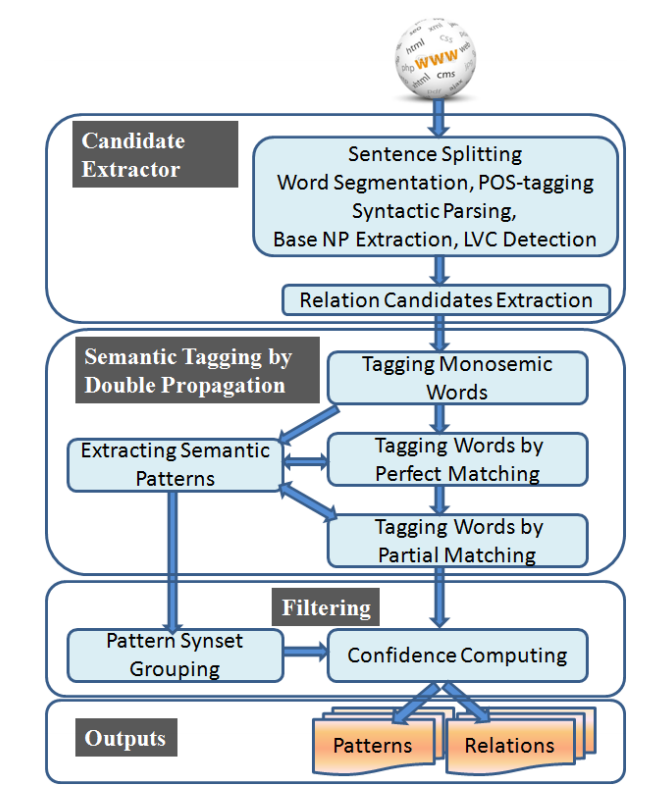
\includegraphics[width=10cm]{ZORE}
\caption{ZORE 体系结构}\label{fig:ZORE}
\end{figure}

\begin{figure}[h]
\centering
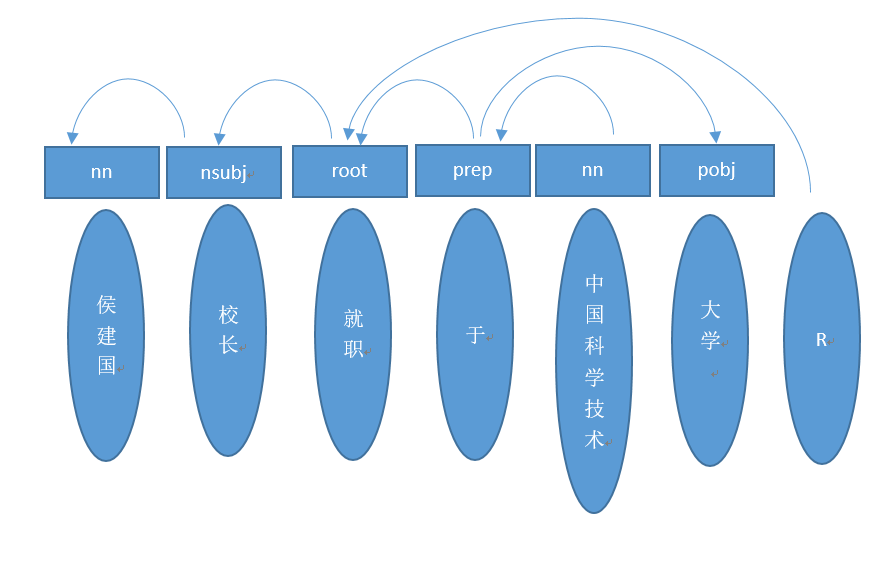
\includegraphics[width=12cm]{parseSentence}
\caption[句子解析结果]{以 StanFord 依存关系对例句“侯建国校长就职于中国科学技术大学”进行解析的结果}\label{fig:parseSentence}
\end{figure}

本文使用的中文语境下的 ORE 系统基于全依存句法分析,并且可以识别涉及长距离依存的模式。鉴于中文的特点,例如缺少功能词\citep{funcword}与形态学\citep{morphword},并且有着较高的词义模糊性与分段性,ZORE 我们将语义本体信息结合到系统的设计中,以提高输出质量,而不会降低效率。

当前使用最新技术的系统是 PAYYT\citep{naka2012},也是基于全依存句法分析,但其为英文语境下的关系抽取系统。并且他们是首先抽取关系再基于抽取的关系对模式进行精细化。ZORE 则将抽取关系与精细化模式同步进行,从而可以让二者互相提升。先前的研究显示模式归纳受益于关系提取\citep{naka2012},并且关系提取也可以受益于模式归纳\citep{mau2012}。通过使用双重拓展算法,不仅可以让模式与关系的提取相互受益,还可以在同一个过程里进行对模式与关系语义类型的标注。

对于中文语境下的关系抽取也有其他的方式,例如基于特征的方法与基于内核的方法。然而,其他的中文语境下的关系抽取都是关注于有着预先定义的关系的传统的信息抽取。语义本体亦是中文语境下的关系抽取里有用的一个定义,却基本没有被使用。并且,那些系统可以被视为一个流水线,依次进行分词、POS 标签标注、解析。ZORE 则给出了语义解释,并通过一种新颖的双重拓展算法在模式和关系之间明确地处理解析中的统计误差。

\section{提取候选关系}

\subsection{解析与基本的 NP 提取}
ZORE 通过应用一系列的 NLP(Natural Language Process,自然语言处理)工具对输入的文本进行流水线处理来分析句法结构。每个句子都通过 Stanford 分割器\citep{chang2008}被分割为一个字词列表,并通过 ZPar \citep{zhang2011}来进行解析,通过标准 CTB \citep{xue2005}来添加 POS 标志和分析结构组成。并对最后生成的构成树使用 Stanford 解析器\citep{chang2008}将其变形为有 Stanford dependencies 的投影树。

接下去,基本的 NPs (名词短语)从依存树中被提取出来,在这里基本 NP 是一个最大短语,其字词只能拥有来自表 ~\ref{tab:NP} 第一行的 POS。

\begin{longtable}{cc}
% 首页表头
\caption[基本 NP 标志表]{包含了 POS 标志和依存标签,在前三行的标签被用来进行基本 NP 的提取,而最后一行中的标签用于从基本 NP 遍历到谓词短语} \label{tab:NP} \\
\toprule[1.5pt]
  & 标志\\
\midrule[1pt]
\endfirsthead
% 续页表头
\caption[]{基本 NP 标志表(续)} \\
\toprule[1.5pt]
  & 标志\\
\midrule[1pt]
\endhead
% 首页表尾
\hline
\multicolumn{2}{r}{\small 续下页}
\endfoot
% 续页表尾
\bottomrule[1.5pt]
\endlastfoot
基本 NP 修饰语   &   NN (common noun), M (measure word), \\
    &   CD (cardinal number), OD (ordinal number),\\
    &   PN (pronoun), NR(proper noun),\\
    &   NT (temporal noun), \\
    &   JJ (other noun-modifier), or PU (punctuation) \\
    \hline
基本 NP 中的标签  &   nn (noun compound modifier), conj (conjunct),\\
    &   nummod (number modifier),\\
    &   cc (coordinating conjunction),\\
    &   clf (classifier modifier), det (determiner),\\
    &   ordmod (ordinal number modifier),\\
    &   punct (punctuation),\\
    &   dep (other dependencies),\\
    &   or amod (adjectival modifier) \\
基本 NP 核心    &   NN (common noun), M (measure word), \\
    &   CD (cardinal number), OD (ordinal number),\\
    &   PN (pronoun), NR(proper noun),\\
    &   NT (temporal noun) \\
    \hline
基本 NP 到谓词的过渡标签  &   nsubj (nominal subject), conj (conjunct),\\
    &   dobj (direct object), advmod (adverbial modifier),\\
    &   prep (preposi-tional modifier),\\
    &   pobj (prepositional object), lobj (localizer object),\\
    &   range (dative object that is a quantifierphrase),\\
    &   tmod (temporal modifier),\\
    &   plmod (localizer modifier of a preposition),\\
    &   attr (attributive), loc (local-izer),\\
    &   top (topic), xsubj (controlling subject),\\
    &   ba (“ba” construction),\\
    &   nsubjpass (nominal passive subject) \\
\end{longtable}

基本 NP 的核心词语可以是一个名词,一个代词,一个数字或是一个量词(表 ~\ref{tab:NP} 的第二行)。基本 NP 里的依存标签只能来自表 ~\ref{tab:NP} 的第三行。所以,很明显的,一个基本 NP 并不包含其他的基本 NP,并且它本身也不被其他的基本 NP 所包含。

\subsection{探测轻量化动词结构}
在语言学中,“轻量化动词”(LVC,light verb construction)指的是一个本身几乎没有语义的动词,并且通常都是和一个名词形成一个谓语\citep{Etzioni2011}。例如,有着“轻量化动词结构”的谓语包括“是国家的”和“宣称拥有主权”,他们的轻量化动词分别是“是”和“宣称”。对 LVC 不合适的处理可能由于不详细的提取导致出现很明显的问题。例如,如果之前两个句子“是国家的”和“宣称拥有主权”中的“是”和“宣称”被作为谓语提取,就会导致提取出的关系无法让人显式地获得有用的信息\citep{Etzioni2011},例如(“税收是国家的收入来源。”,提取出的关系可能是(税收,是,收入来源))。重构动词(ReVerb\citep{Etzioni2011})则解决了以上的问题,通过严格的句法限制让处于动词短语(例如“是”)和介词(例如“的”)中间的名词短语(例如“国家”)被认为是谓词短语的一部分而不是一个论元,从而得出了(税收,是国家的,收入来源)这个关系。

在中文语境中,LVCs 出现的频率非常高,并且应该被妥善地处理,从而保证被提取出的关系可以提供有用的信息。在中文语境中,介词扮演着动词的修饰语,并且可以在动词的左边或右边。例如图 ~\ref{fig:sentence1} 中的例句“侯建国校长就职于中国科学技术大学。”可以被改写为“侯建国校长于中国科学技术大学就职。”,而这两个句子中的介词“于”则分别位于谓词短语“就职”的右边和左边。

中文的 LVCs 可以被归为两类,即“伪 LVC”和“平凡 LVC”。对于伪 LVC,谓词是一个“假的动词”,例如“进行”和“给予”,都是有着名词短语作为他们的对象。因为中文的“假的动词”是一个闭集,我们通过寻找来自语料库的“假的动词”进行探测这种伪 LVC。而对于平凡 LVC,它的谓词则是平凡的动词,即它的谓词有着正常的结构或一个平凡的名词作为对象。例如,“展开调查”就是这种平凡 LVC。

\begin{longtable}{cc}
% 首页表头
\caption[伪 LVC 与平凡 LVC 样例表]{伪 LVC(*) 与平凡 LVC (**)样例表,左列的动词和右列的名词组合生成 LVC,并作为谓词短语。} \label{tab:LVC} \\
\toprule[1.5pt]
动词 & 名词\\
\midrule[1pt]
\endfirsthead
% 续页表头
\caption[]{伪 LVC(*) 与平凡 LVC (**)样例表(续)} \\
\toprule[1.5pt]
动词 & 名词\\
\midrule[1pt]
\endhead
% 首页表尾
\hline
\multicolumn{2}{r}{\small 续下页}
\endfoot
% 续页表尾
\bottomrule[1.5pt]
\endlastfoot
进行(*)   &   发行,分析,收集,修改,访问,处罚\\
    \hline
有(*)  &   影响,贡献,兴趣,帮助,认识,期望\\
    \hline
产生(**)    &   影响,兴趣,怀疑,冲击,好感,恐惧\\
    \hline
造成(**)  &   影响,破坏,伤害,威胁,压力,干扰\\
    \hline
表示(**)  &   满意,欢迎,尊重,担忧,哀悼,感谢\\
    \hline
展开(**)  &   调查,攻击,攻势,批评,批判,诉讼\\
\end{longtable}

平凡 LVC 比伪 LVC 更加难以探测,我们通过上下文的语境来对平凡 LVC 进行探测。包括在 LVC 里的 NP 本身,一个平凡 LVC 通常控制着两个 NP,而处在后面的 NP 则通过一个与 LVC 有关的介词来联系在一起,例如“对,对于,针对,向,同,与,和”。基于以上的现象,一个通用的方法来鉴别平凡 LVC 产生了,即通过寻找在大型语料库中频繁地与 LVC 相关的介词一起出现,被自动解析的动词对象结构。对于一个给定的动词对象 v,用 $f^v$ 和 $f^p$ 分别表示 v 出现的频率和与 v 一起出现的与 LVC 有关的介词的频率。定义 v 成为 LVC 的统计强度为 $f^p / f^v$。如果 v 的统计强度达到了 $t^{lvc}$ 的阈值,则将 v 定义为 LVC。表 ~\ref{tab:LVC} 描述了一些高频率出现的 LVC,通过这种方式被自动提取出来。

\subsection{提取候选关系}
ZORE 尝试从含有两个或更多基本 NP 的句子里抽取候选关系。对于给定的两个基本 NP,我们遍历依存树来获取连结他们的最短路径。而这个最短路径可以仅仅包括表 ~\ref{tab:NP} 中第四行的依存标志,并且必须包括至少一个来自“nsubj”和“dobj”的标志,从而保证这个谓词短语被包括在最短路径中。如果获取到了这样的最短路径,则其他的被同一个谓词短语所控制的基本 NP 也被包括进了这个目标关系里,得出一个 n 元的候选关系,当中的每个基本 NP 都对应着一个论元。依据这个谓词短语,候选关系可以被归为以下几类:

\newtheorem*{CDLR}{平凡与伪 LVC 关系}
\begin{CDLR}
    在这种关系里,最短路径的谓词短语是一个 LVC(例如一个轻量动词和一个普通的对象)。那两个基本的 NP 可以是轻量动词的前置词或子词。以“老李对我的学业有很大帮助”作为例句,“有”和“帮助”结合形成了一个平凡 LVC,并被当成了一个谓词短语,从而得出了关系(老李,Pred[有帮助],我的学业)。
\end{CDLR}
\newtheorem*{VR}{动词关系}
\begin{VR}
    在这种关系里,一个动词则作为一个谓词短语。例如,这个关系(侯建国校长,Pred[就职],中国科学技术大学)提取自图 ~ref{fig:sentence1} 则是一个典型的动词关系。
\end{VR}
\newtheorem*{RCR}{关联从句关系}
\begin{RCR}
    在这种关系里,核心词语是一个名词,被一个关联从句所修饰,并在语义上作为这个关联从句的谓词的论元。“就职于中国科学技术大学的侯建国校长。”这个句子是图 ~\ref{fig:sentence1} 的一个同义句,有着一样的谓词短语和论元。然而,从这个句子里提取出的关系是一个关联从句关系(Pred[就职],中国科学技术大学,侯建国校长),和图 ~\ref{fig:sentence1} 句子的关系属于一样的模式同义词集。
\end{RCR}

\section{双重拓展的语义标注}
基本思想是通过进行对候选关系的论元的核心词语进行词语义标注,迭代地识别关系和模式。对于给定的候选关系集合和语义分类系统,进行拓展包括三个步骤。第一步,候选关系中的单义论元会被用语义类别标注,例如 Af 和 Di,从而获取语义模式。在第二步和第三部,未被标注的的含义模糊和未知词将会分别通过完全匹配和部分匹配进行标注。在每一步的末尾,语义模式来自被提取出和被标注过的关系的概括,之后语义模式被用来帮助下一步的关系标注。因为这种双向的信息交换,这种方式被称之为“双重拓展”。

\subsection{第一步:标注单义的论元}
每个在候选关系内的论元都是基本 NP,因为基本 NP 都是向心结构的\citep{endocentric2017},所以我们可以将一个基本 NP 的核心词语语义类别当作这个基本 NP 的语义类别。在一个分类系统里,每个字词都和一个或更多的语义类别有关。然而,在这步里,只有单义的词语才会被标注,而词义模糊和未知的词语都会被忽略,不会被标注。

大部分被命名的实体并没有被包括在分类系统中。然而,在标注了 POS 标签后,大部分的已命名实体将会被探测为 NR(proper noun,专有名词)。而这导致那些已命名的实体将会被作为词义模糊的词语处理,可以是人名,组织名,或地名。未被分类系统包括的已命名实体将会在第二、三步里被标注。

在这步之后,在一些候选关系里的所有论元都已经被用语义分类标注。这些候选关系被称为“已标注候选关系”,而其他的候选关系则被称之为“未标注候选关系”。已标注候选关系将会被归纳为语义模式,包括句法模式和语义标签,就像图 ~\ref{fig:sentence1} 里所描述的。将由此生成的语义模式称之为$Set^{SemPat}$

\subsection{第二步:完全的模式匹配标注}
在这步,将会通过语义模式匹配对未标注候选关系里的论元进行标注。对于给定的未标注候选关系 r,我们对每一个有着模糊词义的核心词语,获取一个潜在语义类型集合。对于有着未知核心词语的论元,我们根据他们的单字获取潜在语义类型集合。98\% 的中文字词至少都有一个同义字词\citep{qiu2011},并且原字词和同义字词之间至少有一个字一样。对于中文名词,同义字词的集合通常也有着至少一或二个一样的字。所以,对于获取未知字词的潜在的词义类型策略就大致成型了。

首先,对于给定的未知字词 $w^u$,如果我们可以发现一个已知的字词 $w^k$ 与未知的字词 $w^u$ 结尾的两个字一样,则 $w^k$ 的语义类型会被作为 $w^u$ 的潜在语义类型。否则,如果 $w^u$ 和 $w^k$ 最后一个字都一样,那么 $w^k$ 的语义类型会被作为 $w^u$ 的潜在语义类型。

接下去我们开始获取未标注的候选关系的潜在语义标签,这里的未标注候选关系的所有论元已经被潜在语义类型所标注。就像第一步里的,我们将关系 $r$ 归纳为一个句法模式 $pat^{syn}$,之后将 $pat^{syn}$ 与每一个 $r$ 的潜在语义标签来生成潜在语义模式。为了避免一个或更多 $r$ 的潜在语义模式存在于 $Set^{SemPat}$ 中,如果那些语义模式当中频率最高的模式超过了阈值 $t^{sem}$ ,那么符合条件的模式将会被作为 $r$ 的语义模式,由此我们推断 $r$ 的语义标志和之后 $r$ 的每个论元的核心词语的语义类型。做完这步以后,每个语义模式在 $Set^{SemPat}$ 中的频率都会依据最新被标注的候选关系进行更新。

\subsection{第三步:部分的模式匹配标注}
在这步,我们标注含混的和未知的字词,通过部分的匹配而不是完全的整个语义模式的匹配。这被当作一个最后一步的补偿。

我们首先将 $Set^{SemPat}$ 中的一个 n 元语义模式分割为二元语义模式,并计算它们的频率。之后,我们将每个未标注的候选关系 $r$ 分割为几个二元的子关系,并从每一个二元的子关系搜索符合与第二步一样的条件的语义模式。

对于每个二元的子关系,我们获取最高频率的二元语义标志。之后通过结合二元语义标志,我们就可以获取 $r$ 的一个 n 元的语义标签,基于这个语义标签,所有的未知和含混的字词都可以被语义类型所标注。如果一个候选关系 $r$ 的所有的论元已经被标注,那么 $r$ 可以被当作已经被标注。最后,根据最新的被标注的关系,$Set^{SemPat}$ 中的统计数据也将被更新。

\section{将模式分组为同义词集}

\begin{algorithm}[!h]
\SetAlgoLined
\SetKw{KwA}{and}
\SetKw{KwO}{or}
    \uIf{$Pred_i$ = “是” \KwO $Pred_j$ = “是”}{
        \KwRet{$false$}\;
    }
    \uElseIf{$ArgCount(SemPat_i) = 2$ \KwA $ArgCount(SemPat_j) = 2$ \KwA $SemCat(arg_1) = SemCat(arg_2)$}{
        \uIf{$SynPat_i \approx SynPat_j$ \KwA $IsSynonym(Pred_i, Pred_j$) \KwO $Pred_i = Pred_j$}{
            \KwRet{$true$}\;
        }
        \Else{
            \KwRet{$false$}\;
        }
    }
    \uElseIf{$Pred_i = Pred_j$ \KwA $SemSig_i = SemSig_j$ \KwO $IsSynonym(Pred_i, Pred_j)$ \KwA $SemSig_i = SemSig_j$ \KwA $SynPat_i \approx SynPat_j$}{
        \KwRet{$true$}\;
    }
    \Else{
        \KwRet{$false$}\;
    }
\caption[模式同义词集分组]{模式同义词集分组}
\label{algo:grouping}
\end{algorithm}

在这步,我们将来自 $Set^{SemPat}$ 中的语义模式分组为模式同义词集,基于一个单通道的聚类过程\citep{papka1998}。

对于给定的两个语义模式 $SemPat_i$ 和 $SemPat_j$,我们分别以 $SynPat_i$,$SynPat_j$,$SemSIg_i$,$SenSig_i$,$Pred_i$,$Pred_i$ 来表示他们所导出的句法模式、语义标志、谓词短语。在忽略谓词短语的情况下,$SynPat_i$  和 $SynPat_j$ 是完全相同的,并且在这种前提下我们称他们的关系为为约等于($ \approx$)。

算法 \ref{algo:grouping} 的功能为对模式进行分组,其中 $ArgCount(SynPat_i)$ 表示在 $SynPat_i$ 中的论元的数量,$SemCat(Arg_i)$ 表示第 i 个论元的语义类别,而以两个谓词入参的 $IsSynonym(Pred_i, Pred_j)$ 则会得出入参的这两个谓词是否是同义词。

在基于相似性的单通道聚类中,主题偏移的问题十分常见\citep{papka1998}。但是因为这里的相似性测度是均匀的,所以算法 \ref{algo:grouping} 并不会受到主题偏移的影响。

\section{计算关系的置信度}
在没有过滤的情况下,算法 \ref{algo:grouping} 的提取可能产出不正确的关系。根据以前的 ORE 系统,我们可以使用一个置信度的阈值来达到召回与精确之间的平衡。

一种Logistic 回归分类器被用来为每一个关系进行置信度分数的计算,他们的特征值在表 ~\ref{tab:feature} 中展示。在这个表中,$c$,$r$,$arguments$,$SemPat$ 分别表示从句(Clause),关系(Relation),关系中的论元,语义模式(Semantic Pattern)。$Length(r)$,$Count(arguments)$,$Size(SemPat)$ 分别表示 $r$ 中的字数,$r$ 中的论元个数,和 $r$ 的语义模式 $SemPat$ 一样的关系的数量。因为从双重拓展中提取出的语义模式被用作分类器中的特征,所以他们也参与了关系抽取。他们对关系抽取的影响可以直接体现在双重拓展算法的效率中。

\begin{longtable}{ccc}
% 首页表头
\caption[Logistic 回归分类器特征表]{带权重的Logistic 回归分类器特征,通过 Wiki-500 的数据进行训练所得出。} \label{tab:feature} \\
\toprule[1.5pt]
类型 & 特征 & 权重\\
\midrule[1pt]
\endfirsthead
% 续页表头
\caption[]{Logistic 回归分类器特征表(续)} \\
\toprule[1.5pt]
类型 & 特征 & 权重\\
\midrule[1pt]
\endhead
% 首页表尾
\hline
\multicolumn{3}{r}{\small 续下页}
\endfoot
% 续页表尾
\bottomrule[1.5pt]
\endlastfoot
基本(Base)   &   $r$ 覆盖了 $c$ 中所有词语           &   0.96\\
基本(Base)   &   $r$ 中有逗号                        &   -0.47\\
基本(Base)   &   $Length(r) < 10 个字$              &   0.35\\
基本(Base)   &   $10 个字 \leq Length(r) < 20个字$ &   0.11\\
基本(Base)   &   $Length(r) < 20个字$             &   -1.06\\
基本(Base)   &   $Count(arguments) = 2$             &   0.14\\
基本(Base)   &   $Count(arguments) = 3$             &   0.33\\
基本(Base)   &   $Count(arguments) = 4$             &   -0.60\\
基本(Base)   &   $Count(arguments) > 4$           &   -0.46\\
    \hline
词义模式(SemPat)  &   在第三步中被标注                 &  0.87\\
词义模式(SemPat)  &   在第三步前被标注                 &  0.75\\
词义模式(SemPat)  &   $50 \leq Size(SemPat)$且未被标注 &  -0.05\\
词义模式(SemPat)  &   $50 \leq Size(SemPat)$且已被标注 &  0.65\\
词义模式(SemPat)  &   $10 \leq Size(SemPat) < 50$且未被标注 &  -0.16\\
词义模式(SemPat)  &   $10 \leq Size(SemPat) < 50$且已被标注 &  0.39\\
词义模式(SemPat)  &   $5 \leq Size(SemPat) < 10$且未被标注 &  -0.22\\
词义模式(SemPat)  &   $5 \leq Size(SemPat) < 10$且已被标注 &  0.36\\
词义模式(SemPat)  &   $Size(SemPat) < 5$且未被标注 &  -0.92\\
词义模式(SemPat)  &   $Size(SemPat) < 5$且已被标注 &  -0.64\\
\end{longtable}

\section{本章小结}
这一章的内容集中介绍了 ZORE 系统的架构与其对中文文本的关系抽取过程,包括分词、词性标注、依存句法分析、双重拓展算法的介绍和 $Logistic$ 置信度的计算方法,为下一章进行实验做好准备。

  \chapter{实验分析}
本文基于第三章里所提及的 ZORE 系统来进行中文文本的关系抽取。当中包括了 ZORE 在试验的语料库上的运行及其抽取关系实验。本章首先介绍了当前主流的对于开放式关系抽取算法评价指标,之后介绍了如何获取对当前算法评估所需的数据以及将 ZORE 算法与 DPM 算法进行对比,列出并分析了实验结果以及实验中出现的错误出现原因,提出基于实验数据的对 ZORE 进行性能提高设想。
\section{评判标准}对于 ZORE 系统的评判指标,此处使用主流论文对于开放式关系抽取算法的评价指标:准确率(Precision)、召回率(Recall)、综合评价 F1 值。

为了精确地统计 ZORE 系统运行关系抽取功能于各语料库内的性能数据,采用人工对抽取结果进行检查。实验数据的统计方法为:第一步,对 ZORE 算法的抽取结果进行人工标注,判断其求出的关系元组是否符合人的理解方式,若符合,则将该组标注为 $True$,反之则标注为 $False$,$T$ 为全部的有 $True$ 标记的关系元组集,$N$ 则为全部的有 $False$ 标记的关系元组集,$A$ 表示所有被抽取出的关系元组集,$A=T\cup N$。$S$ 则表示人工对语料库标注的实际正确关系集合。
    \begin{equation}
        Precision=\frac{|T|}{|A|}\times 100\%
    \end{equation}
    \begin{equation}
        Recall=\frac{|T|}{|S|}\times 100\%
    \end{equation}
    \begin{equation}
        F1=\frac{2\times Precision\times Recall}{Precision+Recall}
    \end{equation}

显然,Precision 为算法所求得的正确关系元组数占所有关系元组的百分比,算法抽取的关系的正确结果比例随着 Precision 的升高而升高。召回率则表示算法所求出的正确关系占实际正确关系的比例,可以提供算法抽取关系是否全面的评价指标,随着比例增高遗漏实际正确关系的概率会降低。普遍状态下,召回率与精确率成反比,即召回率越高精确率越低,故还有指标 F1 来评价算法的综合性能,显然,F1 越大则算法全面表现越出色。

\section{实验环境构建}
操作系统:Windows10,java version 1.8.0\_131,IDE 使用 Eclipse。在语料库“燃规3”中运行 ZORE。本语料库经过过滤“燃规3”中未以标点符号结尾的句子后,由 331 个句子构成,而中文词典《同义词林》\citep{che2005}则被用来提供每个字词的语义类别。《同义词林》包含了 77492 个中文字词,并被组织为五级的分层。在顶层有 12 个类别,第二、第三层则分别有 94 和 1492 个类别。在 ZORE 系统中以第二层的类别作为语义分类基准。而模式匹配的阈值 $t^{lvc}$ 与 $t^{sem}$ 分别设置为 0.4 与 3。

对于实验文本的数据集,因为是法规类文本,所以需要对每个条目开头的数字编号进行处理,以避免进行关系抽取时这些数字对关系抽取产生影响。因为每个条目开头数字编号的结构是“数字.数字.数字”,即 python 下的正则表达式类型为 $\backslash d\backslash .\backslash d\backslash .\backslash d$。以下为 python 对文本数据的预处理:

\begin{lstlisting}[language=python, caption=python 文本预处理, label={code:pythonpreprocess}]
import re

fo = open("foo.txt", "r")
bar = open("foo_modified.txt", "w")
while 1:
    line = fo.readline()
    if not line:
        break
    line = re.sub("\d\.\d\.\d", "", line)
    bar.write(line)
fo.close()
bar.close()
\end{lstlisting}

对输入文本进行完去除噪声处理之后,便可以开始使用 ZORE 对文本进行处理。处理完成后,ZORE 将文本中抽取出的关系以 $*.xml$ 的方式进行存储,图 ~\ref{fig:result} 表示了 ZORE 从“燃规3”中的一个句子里提取出的关系。

输出的关系文件当中存在 ZPar 依存分析的标签,各标签的含义如表 ~\ref{tab:ZParDep}。

\begin{longtable}{|c|c|c|c|}
% 首页表头
\caption[ZPar 依存分析标签]{ZPar 依存分析的标签} \label{tab:ZParDep} \\
\toprule[1.5pt]
 标签 & 含义 & 标签 & 含义 \\
\midrule[1pt]
\endfirsthead
% 续页表头
\caption[]{ZPar 依存分析的标签(续)} \\
\toprule[1.5pt]
 标签 & 含义 & 标签 & 含义 \\
\midrule[1pt]
\endhead
% 首页表尾
\hline
\multicolumn{4}{r}{\small 续下页}
\endfoot
% 续页表尾
\bottomrule[1.5pt]
\endlastfoot
    ROOT    &   核心关系    &  VOB     &   动宾关系    \\
    \hline
    RAD     &   右附加关系    & RED    &   重复元素    \\
    \hline
    SBV     &   主谓关系     & RADC    &   非共享右附加关系    \\
    \hline
    PUS     &   句中标点      & IOB    &   间宾关系    \\
    \hline
    POB    &   介词宾语      & ACT    &   动词性宾语    \\
    \hline
    ATT    &   定中关系     & ADV    &   状中关系    \\
    \hline
    CMP    &   动补关系      & APP    &   同位语关系    \\
    \hline
    COO    &   并列关系      & COS    &   右共享并列关系    \\
    \hline
    IC    &   独立子句     & IS    &   独立结构    \\
    \hline
    PUN    &   句末标点      &  TPC    &   主题    \\
    \hline
    VV    &   串行动词      & MT    &   时态    \\
    \hline
    NUM    &   数量      & QUN    &   度量关系    \\
    \hline
    QUC    &   前置量词     & QUCC    &   非共享前置量词    \\
    \hline
     ISC    &   非共享独立结构      & LAD    &   左附加关系    \\
\end{longtable}

因为 ZORE 利用 ZPar 进行依存句法分析,所以输出的关系文件当中存在 ZPar 所定义的词性标注的标签,各标签的含义如表 ~\ref{tab:ZParSem}。

\begin{figure}[htb]
\centering
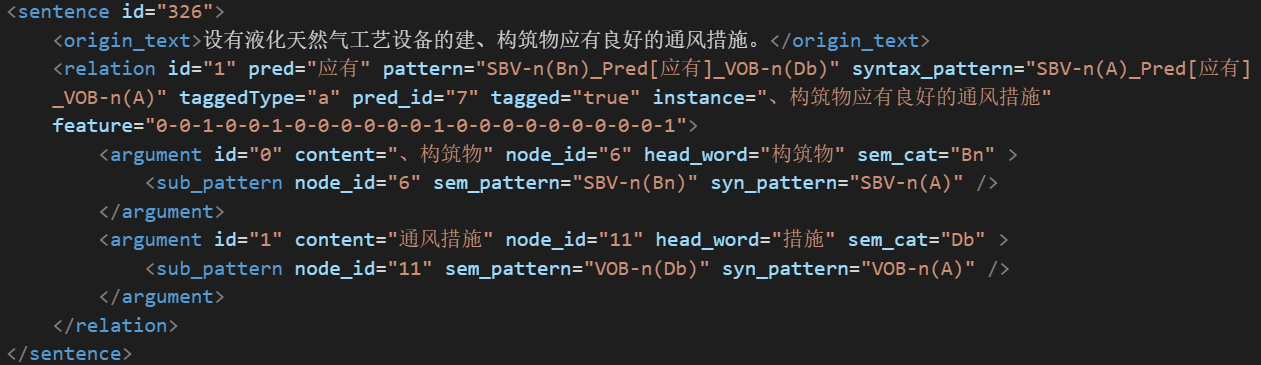
\includegraphics[width=15cm]{result}
\caption{ZORE 的输出}\label{fig:result}
\end{figure}

\begin{longtable}{|c|c|c|c|}
% 首页表头
\caption[ZPar 词性标注标签]{ZPar 词性标注的标签} \label{tab:ZParSem} \\
\toprule[1.5pt]
 标签 & 含义 & 标签 & 含义 \\
\midrule[1pt]
\endfirsthead
% 续页表头
\caption[]{ZPar 词性标注的标签(续)} \\
\toprule[1.5pt]
 标签 & 含义 & 标签 & 含义 \\
\midrule[1pt]
\endhead
% 首页表尾
\hline
\multicolumn{4}{r}{\small 续下页}
\endfoot
% 续页表尾
\bottomrule[1.5pt]
\endlastfoot
    a    &   形容词    &  d     &   副词    \\
    \hline
    c     &   连词    & e    &   感叹词    \\
    \hline
    f     &   方位词     & o    &   拟声词    \\
    \hline
    g     &   语素词      & h    &   前缀成分    \\
    \hline
    i    &   成语      & p    &   介词    \\
    \hline
    q    &   量词     & s    &   所处词    \\
    \hline
    y    &   语气词      & t    &   时间词    \\
    \hline
    v    &   动词       & nrf    &   姓氏    \\
    \hline
    nx    &   非汉语名词     & b    &   区别词    \\
    \hline
    m    &   数词      &  j    &   简称缩写    \\
    \hline
    k    &   后缀成分      & l    &   习语    \\
    \hline
    n    &   名词      & nr    &   人名    \\
    \hline
    ns    &   地名     & nt    &   机构团体    \\
    \hline
     nz    &   其他专名词      & r    &   代词    \\
    \hline
     x    &   非语素词      & z    &   状态形容词    \\
    \hline
     u    &   助词      & w    &   标点    \\
    \hline
     nrg    &   姓      &     &       \\
\end{longtable}

% 而关系(taggedType)则有“a,n,h,t”四种,分别代表“默认的被抽取出的关系,通过相关关系标注,未被标注且已知语义模式,已被标注且已知语义模式”。
feature 为类似于表 ~\ref{tab:feature} 中的对应 feature 的符合关系,其中增加了对于四种 taggedType 的判断,以“1”为符合条件,“0”不符合条件来进行标注。以图 ~\ref{fig:result} 作为句子抽取实例,可以读出,这个句子为语料库中第 326 个句子(sentence id = 326),仅被抽取出一个关系,关系类型为普通,谓词是“应有”(pred = “应有”),语义模式为\{ SBV-n(Bn),Pred[应有],VOB-n(Db) \},查表 ~\ref{tab:ZParDep} 可得前后两个论元的依存类型分别为主谓关系(SBV)和动宾关系(VOB),谓词是句子里从左到右的第七个词汇,语法模式为\{ SBV-n(A),Pred[应有],VOB-n(A) \}。在两个论元里,则提供了其在依存树中的节点序号、核心词汇、内容以及语义类型(sem\_cat),还有其子模式的具体信息。

还可以发现其对语句里关系的抽取遗漏了一个关系(设有液化天然气工艺设备,的,建、构筑物),所以 ZORE 算法对于中文文本的开放式关系抽取并不是完全覆盖的,也就涉及到了下文对于 ZORE 算法的评价以及获取全面、正确的手工标注关系数据集所需要做的工作。

\section{实验结果分析与评价}
本文对被提取出的关系的精确度(Precision)和召回率(Recall)进行评价。一个被提取出的关系仅在谓词短语和其他的所有论元匹配了全部的句中内容才被认为是正确的、有意义的。

对语料库“燃规3”进行中文开放式关系抽取耗费的总时间虽然较长,但其包括读取知识库和对中文语料库进行自然语言处理的 203 秒和对文本进行解析的接近一分钟的时间,可见该系统的运行效率很大程度上受到对中文语料库进行自然语言处理效率不是很高的拖累。可以考虑换用其他类型的自然语言处理工具来替代当前 ZORE 系统中的 StanFord NLP 自然语言处理模块从而帮助提升系统的整体效率。

以人工标注的“燃规3”关系文件 relation-500-human.xml 作为实际正确关系集 $S$,relation-500.xml 作为算法提取出的关系集 $A$,语义模式重复频度阈值的初始值设为 19,以 1 为步长递减至 3,以下为评价程序的工作代码:

\begin{lstlisting}[language=java, caption=评价程序, breaklines=true, label={code:evaluate}]
public static void main(String[]args){
    for(int i=19;i>3;i--){
        EvaluateCORE evaluate=new EvaluateCORE();
        String sHumanTaggedFileName="tagged/relation-500-human.xml";
        String sAutoTaggedFileName="result_origin_rule/relation-500.txt";
        String sOutputFileName="score.txt";
        evaluate.nThresholdSem=i;
        evaluate.filterType="tn";
        System.out.println("evaluate.filterType="+evaluate.filterType);
        String sPatterFileName="result_origin_rule/pattern_synset.txt";
        evaluate.readPatternScore(sPatterFileName,"gbk");
        evaluate.evaluate(sHumanTaggedFileName, sAutoTaggedFileName,sOutputFileName);
    }
}
\end{lstlisting}

其中,evaluate(String sHumanTaggedFileName, String sAutoTaggedFileName, String sOutputFileName) 这个函数是这个评价程序的核心,对 ZORE 输出的关系抽取结果 $sAutoTaggedFileName$ 与人工标注的关系文件 $sHumanTaggedFileName$ 进行比较,$sOutputFileName$ 则记录了了输出的比较数据记录。

对人工标注的关系文件与 ZORE 算法生成的关系文件当中句子逐个按照关系、论元、谓词短语进行比较,此函数调用了 compareTwo(Vector<ExtractedSentence> vecHumanSentence, Vector<ExtractedSentence> vecAutoSentence)。

比较的思想为,首先尝试将人工标注关系与 ZORE 提取出的关系的谓词短语进行匹配测试,若匹配成功则继续进行二者的论元匹配测试;若至少存在一个论元匹配,则自增谓词短语正确数,若所有论元都匹配成功,则自增关系正确数;之后往论元正确数加上当前匹配成功的论元个数,经过以上的处理之后,就得出了计算精确率 Precision 所需的“正确关系数”与“总关系数”。

因为考虑到当前 ZORE 系统所调用的自然语言处理模块不能很好地将以“的”和“是”作为谓词短语的向心结构关系进行分词、依存分析、词性标注,故会影响到 ZORE 系统对其的抽取,这并不是由于 ZORE 算法设计失误导致的抽取缺陷,并且以“的”和“是”作为谓词短语的向心结构关系经过训练集训练之后已经得出是一种高频出现的关系,如果将其包括在内会影响召回率的计算,所以对于召回率 Recall 计算时,人工标注的关系集 $S$ 将以“的”和“是”作为谓词短语的向心结构关系排除在外。

对于语料库的手工标注关系数据集,基于 ZORE 算法所输出的三千多行关系集文件“relation.xml”进行修改。因为评价程序对于关系的评价数据的精确率 Precision 、召回率 Recall 以及由前二者计算出的 F1 值只是基于评价程序中对于谓词短语 predicate、谓词短语的论元内容 arguArr.content 和手工标注关系数据集与 ZORE 生成的关系集文件的二者对应的关系的论元个数 arguArr.size() 来进行匹配。所以在手工标注时无视其他在 ZORE 算法所输出的关系集文件内关系的其他参数,仅仅关注于四个方面:第一,语句当中含有的关系数量,由其 relation id 体现;第二,关系集当中的谓词短语 predicate phrase 是否正确;第三,关系中的论元内容 content 是否正确;第四,关系中的论元个数是否正确。进行多个独立专家标注关系数据集并将其用交叉对比形式保证准确客观性的成本极高,而自己动手进行标注的话可以加深对于自然语言处理及其关系抽取的理解,所以本次进行实验的对 ZORE 输出手工标注关系数据集由作者进行,尽力以客观、简洁的方式审阅 ZORE 算法输出的数据集文件并进行人工标注,从而获得评价 ZORE 算法所需的手工标注关系数据集文件“relation-500-human.xml”。

\begin{longtable}{|c|c|c|c|}
% 首页表头
\caption[ZORE 性能数据]{ZORE 运行于语料库“燃规3”上的性能数据} \label{tab:ZOREperformance} \\
\toprule[1.5pt]
 召回率 & F1 值 & 精确率 & $t^{sem}$\\
\midrule[1pt]
\endfirsthead
% 续页表头
\caption[]{ZORE 运行于语料库“燃规3”上的性能数据(续)} \\
\toprule[1.5pt]
 召回率 & F1 值 & 精确率 & $t^{sem}$\\
\midrule[1pt]
\endhead
% 首页表尾
\hline
\multicolumn{4}{r}{\small 续下页}
\endfoot
% 续页表尾
\bottomrule[1.5pt]
\endlastfoot
0	&	0	&	1	&	19\\
    \hline
0.02	&	0.039111111	&	0.88	&	18\\
    \hline
0.05	&	0.094117647	&	0.8	&	17\\
    \hline
0.1	&	0.178494624	&	0.83	&	16\\
    \hline
0.14	&	0.24040404	&	0.85	&	15\\
    \hline
0.2	&	0.323809524	&	0.85	&	14\\
    \hline
0.245	&	0.383288889	&	0.88	&	13\\
    \hline
0.294	&	0.435555556	&	0.84	&	12\\
    \hline
0.343	&	0.483680138	&	0.82	&	11\\
    \hline
0.392	&	0.526174497	&	0.8	&	10\\
    \hline
0.4394	&	0.562132196	&	0.78	&	9\\
    \hline
0.4532	&	0.565559907	&	0.752	&	8\\
    \hline
0.4743	&	0.574383099	&	0.728	&	7\\
    \hline
0.4876	&	0.557208158	&	0.65	&	6\\
    \hline
0.5358	&	0.576546301	&	0.624	&	5\\
    \hline
0.5674	&	0.574899548	&	0.5826	&	4\\
    \hline
0.6193	&	0.545454545	&	0.512	&	3\\
\end{longtable}

\begin{figure}[t]
\centering
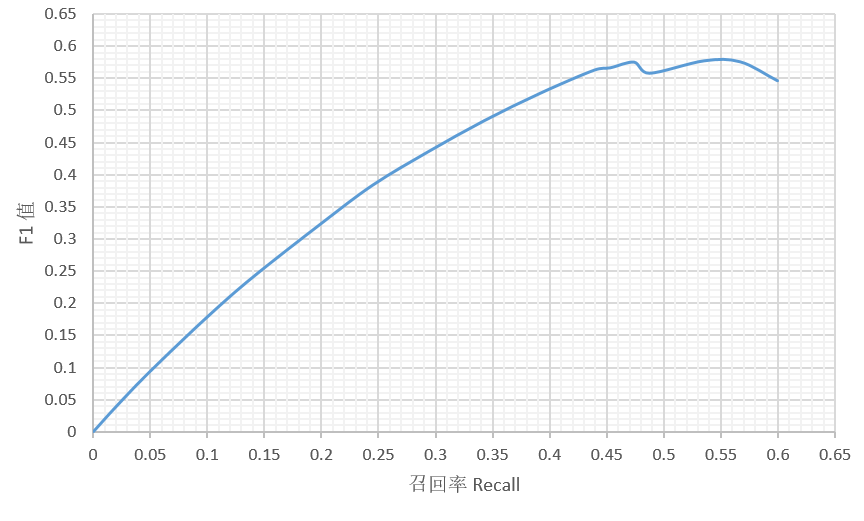
\includegraphics[width=15cm]{performance}
\caption[ZORE 性能图]{ZORE 基于语料库“燃规3”的 F1 值}\label{fig:performance}
\end{figure}

评价程序数据生成的算法性能图 ~\ref{fig:performance} 以 F1 值作为 ZORE 算法综合性能的评价,下表为基于运行评价程序所得出的数据。可以看出,随着词性过滤阈值 $t^{sem}$ 的下降,算法的召回率 Recall 不断提高,而精确率 Precision 却在不断下降,对算法的综合性能衡量指标 F1 值则上下浮动,大体上呈现一种多次函数的模式。

图 ~\ref{fig:performance} 显示了在不同的召回率下 ZORE 在“燃规3”数据集中的表现。体现了先前提及的对召回率 Recall 与精确度 Precision 的平衡性权衡,即 F1 的值先是随着召回率 Recall 的增加而增加,到达极大值后开始下降,则选择 F1 拥有极大值处的召回率 Recall 值可以获得当前语料库下 ZORE 算法的最佳综合性能表现。

同时,以另一种开放式关系抽取算法 DPM\citep{liyang2016} 来与 ZORE 的性能进行比较。二者之间最大的区别就是 DPM 算法增加了对于兼类词的探测和处理,使词性标注出现错误的概率降低,从而提升关系抽取的精确性 Precision,其余处理部分大体相同,也可称之为 ZORE 的兼类词处理版本。

\begin{figure}[h!]
\centering
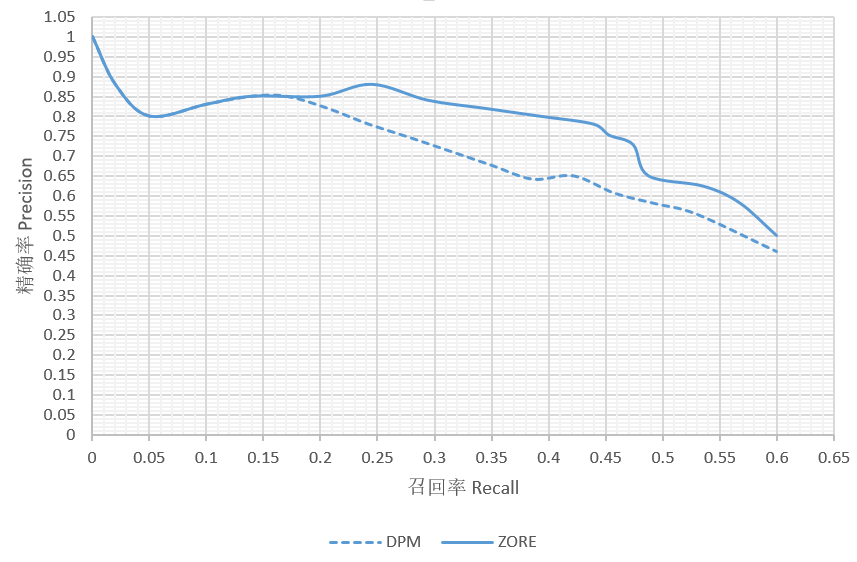
\includegraphics[width=15cm]{compare}
\caption{ZORE 与 DPM 的 P-R 曲线对比}\label{fig:compare}
\end{figure}

\begin{longtable}{|c|c|c|c|}
% 首页表头
\caption[DPM 性能数据]{DPM 运行于语料库“燃规3”上的性能数据} \label{tab:DPMperformance} \\
\toprule[1.5pt]
 召回率 & F1 值 & 精确率 & $t^{sem}$\\
\midrule[1pt]
\endfirsthead
% 续页表头
\caption[]{DPM 运行于语料库“燃规3”上的性能数据(续)} \\
\toprule[1.5pt]
 召回率 & F1 值 & 精确率 & $t^{sem}$\\
\midrule[1pt]
\endhead
% 首页表尾
\hline
\multicolumn{4}{r}{\small 续下页}
\endfoot
% 续页表尾
\bottomrule[1.5pt]
\endlastfoot
0	&	0	&	1	&	19\\
\hline
0.02	&	0.039111111	&	0.88	&	18\\
\hline
0.05	&	0.094117647	&	0.8	&	17\\
\hline
0.1	&	0.178494624	&	0.83	&	16\\
\hline
0.14	&	0.24040404	&	0.85	&	15\\
\hline
0.17	&	0.283333333	&	0.85	&	14\\
\hline
0.206	&	0.329278752	&	0.82	&	13\\
\hline
0.242	&	0.369393346	&	0.78	&	12\\
\hline
0.278	&	0.405152895	&	0.746666667	&	11\\
\hline
0.314	&	0.435742606	&	0.711666667	&	10\\
\hline
0.35	&	0.461363636	&	0.676666667	&	9\\
\hline
0.386	&	0.48203049	&	0.641666667	&	8\\
\hline
0.422	&	0.511753731	&	0.65	&	7\\
\hline
0.458	&	0.521830254	&	0.606333333	&	6\\
\hline
0.494	&	0.533556797	&	0.58	&	5\\
\hline
0.53	&	0.5415749	&	0.553666667	&	4\\
\hline
0.5931	&	0.520754717	&	0.464	&	3\\
\end{longtable}

\begin{figure}[h!]
\centering
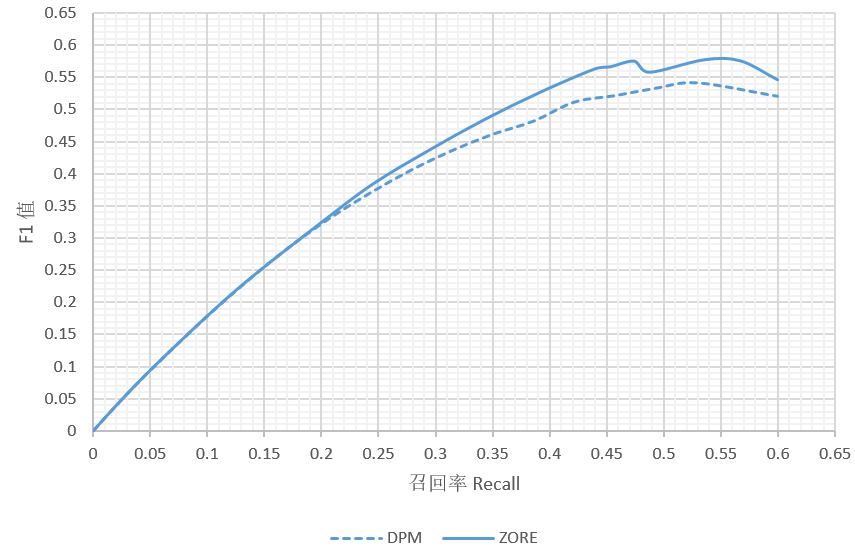
\includegraphics[width=15cm]{comparef}
\caption{ZORE 与 DPM 的 F1 值对比}\label{fig:comparef}
\end{figure}

为了对比的公正客观性,也以“燃规3”作为其语料库进行处理。图 ~\ref{fig:compare} 即为二者运行于同一语料库上的对比图表,可见在特定召回率 Recall 区间上,DPM 精确度 Precision 劣于 ZORE 算法,推断是是由于该语料库是法规,文本结构较为碎片化,以上下文环境进行分析的兼类词处理难以顺利工作导致的。

二者的 P-R 曲线都是体现了精确率 Precision 与召回率 Recall 成反比关系。以及二者之间 F1 值在各种召回率 Recall 下的表现,如图 ~\ref{fig:comparef} 所示,可以看出 DPM 与 ZORE 之间的 F1 值区别并不大,所以可以推断,仅仅增加了对于兼类词处理模块的改进 ZORE 算法得到的 DPM 并没有本质上的提升,即缺少对兼类词处理不是 ZORE 算法提升性能所遇到的瓶颈。

本文经过 ZORE 对语料库“燃规3”进行关系抽取之后,得到了“type\_new.txt”这个所提取出的关系模式统计文件,当中包括了 30 个关系模式及其在训练数据集当中出现的频次和在当前所处理的语料库中出现的频次,以 20 次作为高频出现的阈值,这 30 个关系模式中存在 3 个高频关系模式,分别为:Pattern(nsubj-m(Dn), Pred[de], dobj-n(Di)),22 次;Pattern(nsubj-n(A0), Pred[de], dobj-n(A1)),38 次;Pattern(nsubj-q(Dn), Pred[de], dobj-n(Di)),21 次。很显然,这三个模式都是以“的”为谓词短语的关系模式,与现实生活里的经验符合:由“的”构成的三元组关系模式占正常生活里中文语境下的文本的大多数。

\section{错误分析}
在观察了输出的结果文件后,对不正确的提取(由于精确度的损失)与遗漏的正确的关系(由于召回的损失)进行了统计,得出约 $40\%$ 的遗漏关系是因为语义模式的最低频率限制所导致,而对于语义模式最低频率的限制则是用来平衡召回率与精确率的。

还有一个主要的错误原因是由于解析错误导致的对谓词短语的错误鉴别,带来了全部错误中约 $37\%$ 的报错。也存在由于自然语言处理工具所导致的错误,有分词、依存句法、词性标记等方面产生的错误,例如图 ~\ref{fig:result} 中 argument id = 0 的论元应为 “建、构筑物”而不是“、构筑物”。

这个分词错误也导致了 ZORE 对 id = 326 的句子进行关系抽取时产生了遗漏,关系(设有液化天然气工艺设备,的,建、构筑物)应该在分词正确的前提下被抽取出来。分词错误还会导致对论元的归纳错误,进而影响对 feature 匹配的计量,无法对当前进行分析的句子通过所符合的 feature 数量进行正确的置信度计算,最终影响关系的置信度权重值,使 $Logistic$ 回归分类器无法以当初所预计的工作效果继续工作。

在进行关系提取的过程中也存在选择了错误的模式进行抽取以及未找到可以进行匹配的模式的问题,举个例子,“为使城镇燃气工程设计符合安全生产、保证供应、经济合理和保护环境的要求,制定本规范。”这个句子就未搜索到可以和他匹配的模式进行关系抽取,进而遗漏了(使城镇燃气工程设计,符合,安全生产、保证供应、经济合理和保护环境的要求,制定,本规范),(安全生产、保证供应、经济合理和保护环境,的,要求)这两个关系。

分析结果表明,ZORE 的提取所得到的模式精确率与全面率还有待提升,另外,经过分析可以得出:自然语言处理的工具的性能是提升开放式关系提取算法的瓶颈,句法分析的提升和更加全面且精确的分词系统有很大的可能性让开放式关系抽取也随之进步,所以进行深入研究关于自然语言的处理也是提升开放式关系抽取系统效率的方法之一。亦可追加关系元组进入关系知识库当中,以增加匹配面,故也可对知识库的应用加以研究。

\section{本章小结}
这一章完成了基于特定语料库的算法运行,并对算法的运行结果进行了分析,根据经典的对开放式关系抽取系统的评价标准 P-R 图衡量了算法 ZORE 的综合性能,并验证了词性标签阈值 $t^{sem}$ 对 P-R 图的影响、P-R 二者之间成反比的关系与其权衡。

将 ZORE 与其拥有兼类词处理版本的算法 DPM 进行对比,分析并得出了兼类词处理对于中文开放式关系抽取系统的精确率 Precision 的影响推论。

对于 ZORE 系统的改进,提出了加强系统所使用自然语言处理模块的性能,包括其分词、词性标注、依存句法分析的准确性提高;向关系知识库中追加新的关系元组以增大匹配面;添加对模式进行筛选的算法从而提高对其鉴别的准确性和其对语料库的覆盖率等未来研究方向的设想。
  %自行添加
  %\include{chapter/...}

%%%%%%%%%%%%%%%%%%%%%%%%%%%%%%
%% 附件部分
%%%%%%%%%%%%%%%%%%%%%%%%%%%%%%
\backmatter

  % 参考文献
  % 使用 BibTeX
  % 选择参考文献的排版格式。注意ustcbib这个格式不保证完全符合要求,请自行决定是否使用
  \bibliographystyle{ustcbib}%{GBT7714-2005NLang-UTF8}
  \bibliography{bib/tex}
  \nocite{*} % for every item
  % 不使用 BibTeX
  % \include{chapter/bib}

  % 附录,没有请注释掉
  % \begin{appendix}
  %   
\chapter{中国科学技术大学研究生学位论文撰写规范}
\label{chap:requires}
\section*{以下文字仅作示例,一切以学校规定为准!}
研究生院规定在此下载\url{http://gradschool.ustc.edu.cn/ylb/material/xw/wdxz/1.doc}

研究生学位论文集中反映研究生在研究工作中所取得的成果,代表研究生研究工作的水平,也是申请和授予相应学位的主要依据。为提高研究生学位论文的撰写质量,做到学位论文在内容和格式上的规范化,我们编写了《中国科学技术大学研究生学位论文撰写规范》,供申请学位的研究生参考执行。其中参考文献著录规则我们根据GB/T 7714-2005的标准撰写。硕士和博士学位论文除在研究深度等方面要求不同外,撰写要求基本一致。

\section{内容要求}

\subsection{封面} 
采用研究生院规定的统一封面,封面包含内容如下: 
\subsubsection{密级} 涉密论文必须在论文封面标注密级(内部、秘密、机密),同时注明保密年限。
\subsubsection{论文题目} 应准确概括整个论文的核心内容,简明扼要,最多不超过30字,必要时可以加副标题。
\subsubsection{作者姓名} 英文封面中按英文习惯书写,即名在前。姓名需写全拼。
\subsubsection{学科专业} 写所在专业的全称,不可用简写。
\subsubsection{导师姓名} 一般允许有两名指导教师,主要指导教师姓名写在第一位,后附其职称,次要指导教师排第二位,也需注明职称。
\subsubsection{完成时间} 填写论文打印成文的年月日。

\subsection{中国科学技术大学学位论文原创性和授权使用声明}
本部分内容使用统一的模版,具体内容见格式范例,提交时作者须亲笔签名。

\subsection{摘要和关键词}
\subsubsection{中文摘要}
摘要是论文内容的总结概括,应简要说明论文的研究目的、基本研究内容、研究方法、创新性成果及其理论与实际意义,突出论文的创新之处。不宜使用公式、图表,不标注引用文献。 
\subsubsection{中文关键词} 
关键词是为了文献标引工作从论文中选取出来用以表示全文主题内容信息的单词和术语,一般3--8个词,要求能够准确概括论文的核心内容。
\subsubsection{英文摘要与关键词}
以中文书写的论文,内容与中文摘要和关键词完全一致,其他语种书写的论文以简略为原则,不需要相同。

\subsection{目录}
目录页由论文的章、条、附录等序号、名称和页码组成。论文中如图表较多,可以分别列出清单置于目次页之后。图的清单应有序号、图题和页码。表的清单应有序号、表题和页码。

\subsection{符号说明}
如果论文中使用了大量的物理量符号、标志、缩略词、专门计量单位、自定义名词和术语等,应编写成注释说明汇集表。若上述符号等使用数量不多,可以不设此部分,但必须在论文中出现时加以说明。

\subsection{正文}
正文是学位论文的主体,包括绪论、论文主体及结论等部分。
\subsubsection{绪论}
内容应包括:选题的背景和意义,文献综述及研究现状,研究内容与预期结果,研究方法和实验设计,论文结构安排等。要求实事求是,不夸大、缩小前人的工作和自己的工作,言简意赅,突出重点,不与摘要雷同。
\subsubsection{论文主体}
论文主体是正文的核心部分,占主要篇幅,它是将学习、研究和调查过程中筛选、观察和测试所获得的材料,经过加工整理和分析研究,由材料而形成论点。由于各学科及具体选题的差异,此部分不作统一规定。但总体内容必须实事求是,客观真切,准确完备,合乎逻辑,层次分明,简练可读。
\subsubsection{结论}
结论是对整个论文主要成果的总结,应明确、精炼、完整、准确。其中应明确指出本研究的创新点,对论文的学术价值和应用价值等加以预测和评价,说明研究中尚难解决的问题并提出今后进一步在本研究方向进行研究工作的设想或建议。

\subsection{参考文献}
本着以严谨求实的科学态度撰写论文,凡学位论文中有引用或参考、借用他人成果之处,均应详细列出所引文献的名称、作者、发表刊物、发表时间、卷号、页码等,严禁抄袭剽窃。  
\subsection{附录}
主要列入正文内过分冗长的公式推导,供查读方便所需的辅助性数学工具或表格,重复性数据图表,论文使用的缩写,程序全文及说明等。

\subsection{致谢}
对给予各类资助、指导和协助完成研究工作以及提供各种对论文工作有利条件的单位及个人表示感谢。致谢应实事求是,切忌浮夸与庸俗之词。

\subsection{在读期间发表的学术论文与取得的其他研究成果}
按学术论文发表的时间顺序,列齐本人在攻读学位期间发表或已录用的学术论文清单(发表刊物名称、卷册号、页码、年月及论文署名、作者排序)。其他研究成果可以是申请的专利、获得的奖项及完成的项目等。
 
\section{书写规定}

\subsection{论文的字数要求}
硕士学位论文要求不少于3万字,博士学位论文要求不少于5万字。

\subsection{文字、标点符号和数字}
除留学生和外语专业研究生外,学位论文一律用汉字书写。除非特殊需要,不得使用已废除的繁体字、异体字等不规范汉字。标点符号的用法以GB/T 15834—1995《标点符号用法》为准。数字用法以GB/T 15835—1995《出版物上数字用法的规定》为准。

留学生的学位论文所采用语种可以和导师商定,但论文封面须用中文。

\subsection{封面与扉页}
\subsubsection{秘级} 封面的秘级可以标注为内部、秘密和机密,各密级的保密时限分别为小于等于5年、小于等于10年和小于等于20年,非保密论文不标注密级。
\subsubsection{题目} 题目中避免使用缩略词、首字母缩写字、字符、代号和公式等。
\subsubsection{日期} 封面的日期用汉字书写。
\subsubsection{扉页} 扉页的内容与封面一致。扉页后,需给出英文的封面。其他语种书写的论文还需在英文封面后附上正文所用语种书写的封面。

\subsection{目录}
目录应包括论文的全部内容,包括中英文摘要和附录等,正文章节题名要求编到第3级标题,即×.×.×。一级标题顶格书写,二级标题缩进一个汉字符位置,三级标题缩进两个汉字符位置。

\subsection{摘要与关键词}
\subsubsection{摘要}
摘要分中文和英文两种,中文在前,英文在后。标题摘要二字中间空一格。摘要的字数,硕士学位论文建议1000字以内,博士学位论文建议3000字以内。留学生用其他语种撰写学位论文时,中文摘要应不少于6000汉字。摘要中不得出现图片、图表、表格或其他插图材料。英文摘要与中文摘要应完全一致。
\subsubsection{关键词}
关键词以显著的字符另起一行并隔行排列于摘要下方,左顶格。中文关键词间空一格,英文关键词间用逗号隔开。

\subsection{论文正文}
\subsubsection{章节及各章标题}
论文正文分章节撰写,每章应另起一页。

各章标题字数一般应在15字以内,不使用标点符号。标题中尽量不采用英文缩写词,对必须采用者,应使用本行业的通用缩写词。
\subsubsection{序号}
\paragraph{标题序号}
论文标题分层设序。层次以少为宜,根据实际需要选择。各层次标题一律用阿拉伯数字连续编号;不同层次的数字之间用小圆点“.”相隔,末位数字后面不加点号,如“1”,“1.1”,“1.1.1”等;各层次的序号均左起顶格排,后空1个字距接排标题。例如:

第1章 ××××(大标题) 

1.1 ××××(一级节标题)

1.1.1 ××××(二级节标题)

1.1.1.1 ××××(根据需要,也可设三级节标题)

第2章 ××××(大标题)

2.1 ××××(一级节标题)

2.1.1 ××××(二级节标题)

\paragraph{图表等编号} 
论文中的图、表、附注、公式、算式等,一律用阿拉伯数字分章依序连续编码。其标注形式应便于互相区别,如:图 l.1(第1章第一个图)、图2.2(第二章第二个图);表3.2(第三章第二个表)等。
\paragraph{页码}
页码从绪论开始按阿拉伯数字(1,2,3……)连续编排,此前的部分(中英文摘要、目录等)用大写罗马数字(I,II,III…)单独编排,页码位置居于页脚居中。封面、扉页、创新性声明等不编页码。
\subsubsection{页眉}
页眉从中文摘要开始,内容与该部分的一级标题相同,奇偶页相同,各部分的首页也需有页眉。
\subsubsection{名词和术语}
科技名词术语及设备、元件的名称,应采用国家标准或部颁标准中规定的术语或名称。标准中未规定的术语要采用行业通用术语或名称。全文名词术语必须统一。一些特殊名词或新名词应在适当位置加以说明或注解。

采用英语缩写词时,除本行业广泛应用的通用缩写词外,文中第一次出现的缩写词应该用括号注明英文原词。
\subsubsection{量和单位}
量和单位要严格执行GB 3100~3102-93(国家技术监督局1993-12-27发布,1994-07-01实施)有关量和单位的规定。

量的符号一般为单个拉丁字母或希腊字母,并一律采用斜体(pH例外)。为区别不同情况,可在量符号上附加角标。 

在表达量值时,在公式、图、表和文字叙述中,一律使用单位的国际符号,且无例外地用正体。单位符号与数值间要留适当间隙。具体可参见下列表达式3.1。

\subsubsection{图和表}
\paragraph{图}
图应具有“自明性”,即只看图、图题和图例,不阅读正文,就可理解图意。每一图应有简短确切的题名,连同图号置于图下。

图的位置在相关说明文字之后,随文排。坐标比例不宜过大,同一图上不同曲线的点要分别用不同形状的标识符标出。图中的术语、符号、单位等应与正文表述中所用一致。

图题应简明。图号和图题间空1个字符位置,居中排于图的下方。

必要时,应将图上的符号、标记、代码,以及实验条件等,用最简练的文字,横排于图题下方,作为图例说明(图注)。

\paragraph{表}
表的位置也在相应说明文字之后,随文排。表中参数应标明量和单位的符号。表应有自明性。每一表应有简短确切的题名,连同表号置于表上,表号与表题间空一个字符位置。表号用阿拉伯数字分章编号,如第3章第2个表的表号表示为“表3.2”。

表格太大需要转页时,需要在续表上方注明“续表”,表头也应重复排出。

必要时应将表中的符号、标记、代码,以及需要说明事项,以最简练的文字,横排于表题下,作为表注。相关要求同于图注。

\subsubsection{表达式}
表达式主要指数字表达式,也包括文字表达式。表达式需另行起排,原则上应居中,用阿拉伯数字分章编号。序号加圆括号,右顶格排。例如,第3章第1个表达式:

较长的式如必须转行,只能在+,-,×,÷,<,>处转行,序号编于最后一行的最右边。

\subsection{参考文献}
参考文献参照GB/T 7714-2005《文后参考文献著录规则》执行。推荐使用著者-出版年制,即在正文引用文献处标注著者姓名与出版年份,在文后的参考文献表中标注参考文献的详细信息。
\subsubsection{著者-出版年制在正文中的标注方式}

正文中的标注方式分两种:其一,正文里已出现著作者姓名的,在其后用圆括号附上出版年份即可;其二,正文里仅提及有关的资料内容而未提到著作者,则在相应文句处用圆括号标注著作者姓名和出版年份,两者之间加逗号。

例如:

Park et al(1995)根据Laurentia西缘放射状基性岩墙的研究以及与地幔柱有关的澳大利亚Gairdner岩墙群的研究,首次提出约780Ma地幔柱导致Rodinia超大陆的裂解。

其中关于成冰系顶底界时限和冰川活动年龄、超大陆裂解的起始时间和持续时间……是当前中国地球科学界十分活跃并得到迅速发展的研究领域(王平,2003)。

引用同一著者在同一年份出版的多篇文献时,在出版年份之后用英文小写字母a、b、c……区别。如:(王平,2005a);(王平,2005b)

多处引用同一著者的同一文献时,在“()”外以角标的形式著录引文页码。引用有两个以上同姓的著者的外文文献时,则著者要加名字的缩写,但不必加缩写点。

引用多位著者的文献时,对欧美著者只需标注第一个著者的姓,其后附“et al”,仅两位作者的也可全部注出,中间用“and”;对中国著者应该标注第一著者的姓名,其后附“等”字,姓名与“等”字之间留1个空格。例如:……(王平 等,2005) ……。

同一处引用多篇文献时,按出版年份由近及远依次标注,中间用逗号分开。

\subsubsection{著者-出版年制参考文献表的编排}
 参考文献表加居中标题——“参考文献”,并列入全书目录。

凡正文里括注了著者姓名和年份的,其文献都必须列入参考文献表。

参考文献表中的条目(不排序号),先按语种分类排列,语种顺序是:中文、日文、英文、俄文、其他文种。然后,中文和日文按第一著者的姓氏笔画排序,中文也可按汉语拼音字母顺序排列,西文和俄文按第一著者姓氏首字母顺序排列。

在参考文献中,当一个著者有多篇文献并为第一著作者时,他单独署名的文献排在前面(并按出版年份的先后排列),接着排他与其他人合写的文献。

著录项目与GB/T 7714-2005《文后参考文献著录规则》中规定的顺序编码制基本相同,不同的仅为出版年份排于编著者之后。
\subsubsection{参考文献标注的注意事项}
编著者姓名,一律姓在前、名字在后。西文和俄文的姓全部著录,名字可用大写首字母(不加缩写点);如果姓和名的首字母相同,便要用全名。

以机构和团体署名的文献,此机构或团体可作为编著者,但要用全称,而不用简称或缩写。

编著者不明的文献,编著者一项应注明“佚名”,或用其他与之相应的词。 

编著者为3人以下时全部著录,用逗号分隔,3人以上可只著录前3人,后加“,等”,外文用“,et al”,“et al”不必用斜体。

外文文献大写字母的使用要符合文种本身的习惯用法。

外文期刊刊名可列出全名,也可列惯用缩写刊名(缩写点可加,也可不加,但全文要统一)。只有一个词的刊名不能缩写。期刊名排正体。

期刊只列出卷号,不必标“卷”或“Vol”等;如果是分卷图书,则应加“卷”或“册”或“Vol”或其他语种相应的词(外文缩写词不加缩写点,首字母大小写应全文统一)。

参考文献的版次、卷、期、页码等数字一律用阿拉伯数字表示。版次中中文版次著录为“第2版”、“第3版”……(第1版不必列出),西文文献的版次著录为“2nd ed”、“3rd ed”或其他语种相应的词 。

出版年采用公元纪年,并用阿拉伯数字著录。如有其他纪年形式时,将原有的纪年形式置于“( )”内。

如:1947(民国三十六年)

日文文献中的汉字要用日文汉字。

参考文献中使用的标点符号:

,用于多著者姓名之间,出版者和年或卷(期)之间,期刊名和年或卷之间,“等”或“译”字、专利号等之前。

:用于副题名之前、出版地之后,或引文页码、析出文献页码、专利国别前。

()用于期号、报纸的版次、电子文献更新或修改日期以及非公元纪年。

[] 用于序号、文献类型、电子文献的引用日期以及自拟的的信息。

∥用于专著中的析出文献的出处项前。

- 用于起讫序号和起讫页码间。

. 用于其余各项目之后。

\subsubsection{顺序编码制的著录规则}
参考文献如果按照顺序编码制著录,可参照GB/T 7714-2005《文后参考文献著录规则》执行。


\section{排版和印刷要求}略

\chapter{关于规范本科毕业论文(设计)格式和统一封面的通知}
\section*{以下文字仅作示例,一切以学校规定为准!}
教务处规定在此下载\url{http://202.38.70.92/bklw.doc}

\hspace{-2em}各院系:

鉴于目前各院系本科毕业论文(设计)存在着论文格式不够规范、封面不统一的状况,为加强本科毕业论文的管理,提高论文质量,同时规范全校本科毕业论文(设计)格式,现对本科毕业论文格式和统一封面规定如下:
\begin{enumerate}
\item 本科毕业论文按编排顺序应包括以下内容:封面、扉页、致谢、目录、中文内容摘要、英文内容摘要、正文章节、参考文献或资料注释、附录等。
\item 本科毕业论文的格式要求:
\begin{enumerate}
\item 封面中“论文题目”等内容用四号宋体。
\item 除封面、扉页外,每面上部加页眉,用小5号字标注“中国科学技术大学本科毕业论文”,居中。
\item 从目录页开始在每面底部居中用小五宋体连续编页码。
\item 论文的“致谢”、“目录”等标题用小二号黑体字,居中。
\item 目录一般列三级,后附规范的页号。
\item 正文中的标题分章、节、段三级;章、节标题居中,段标题居左,分别用三号黑体、小三黑体、四号黑体。
\item 具体内容用小四号宋体,每行间距为22磅,科学公式和符号要符合国标,公式要单独占行、居中、行距为单倍行距。
\item 表格、插图全文要分别统一编号或按章编号,标题用小四宋体:(表格标题居表上方,插图标题居图下方),居中。
\item 参考文献的内容包括:序号、作者名、书名或文章名、刊物名或出版社名、
刊物期卷、页和日期,用小四宋体,外文期刊名用白斜体。
\item 附录为:
\begin{enumerate}
\item 重要参考文献中相关内容和章节复印件;
\item 作者或导师所做的与本论文有关的成果复印件。
要求用A4纸复印附于参考文献后。
\end{enumerate}
\end{enumerate}
\item 本科毕业论文(设计)封面学校已统一印制,请到教材科领购。
\item 装订要求:每份论文必须用A4纸打印(复印)、装订成册(教材科可提供复印、装订业务)。另外,校级优秀毕业论文必须提交一份线装毕业论文交档案馆收藏。
\item 具体格式详见附件式样。
\end{enumerate}
\begin{flushright}
中国科技大学教务处

二OO二年三月二十八日
\end{flushright}
附件:本科毕业论文(设计)式样

(略)

  % \end{appendix}

  \makeatletter
  \ifustc@bachelor\relax\else
    % 致谢
	
\begin{thanks}

在中国科技大学完成本科学业的四年里,我所从事的学习和研究工作,都是在导师以及系里其他老师和同学的指导和帮助下进行的。在完成论文之际,请容许我对他们表达诚挚的谢意。

感谢班主任王海龙老师多年的关怀。感谢蒋凡等老师,他们本科及研究生阶段的指导给我研究生阶段的研究工作打下了基础。

感谢张练钢等师兄师姐们的指点和照顾;感谢李卓华等几位同班同学,与你们的讨论使我受益良多;感谢王译锋等师弟师妹,我们在实验室共同学习共同生活,一起走过了这段愉快而难忘的岁月。

感谢科大,感谢一路走过来的兄弟姐妹们,在最宝贵年华里,是你们伴随着我的成长。

最后,感谢我家人一贯的鼓励和支持,你们是我追求学业的坚强后盾。

\vskip 18pt

\begin{flushright}

曾锃煜

\today

\end{flushright}

\end{thanks}
%硕博致谢部分
    % 发表文章目录
    \include{chapter/pub}
  \fi
  \makeatother

\end{document}
